\section{三点共线与三线共点}
%---------------------------------------------------
\subsection{梅涅劳斯定理}
\begin{theorem}[梅涅劳斯(Menelaus)定理]
    如果一条不通过A、B、C三点的直线与$\triangle ABC$ 的边BC、CA、AB所在直线分别交于X、Y、Z,则 
    $$\frac{A Z}{Z B} \cdot \frac{B X}{X C} \cdot \frac{C Y}{Y A}=1.$$ 
\end{theorem}


\begin{figure}[htbp]
    \centering
    \hfill % 添加一些水平间距
    \begin{minipage}[t]{0.45\textwidth}
        \centering
        \includegraphics[width=\linewidth]{figures/menelaus.png}
        % \caption{情形1}
    \end{minipage}
    \hfill % 添加一些水平间距
    \begin{minipage}[t]{0.45\textwidth}
    \centering
    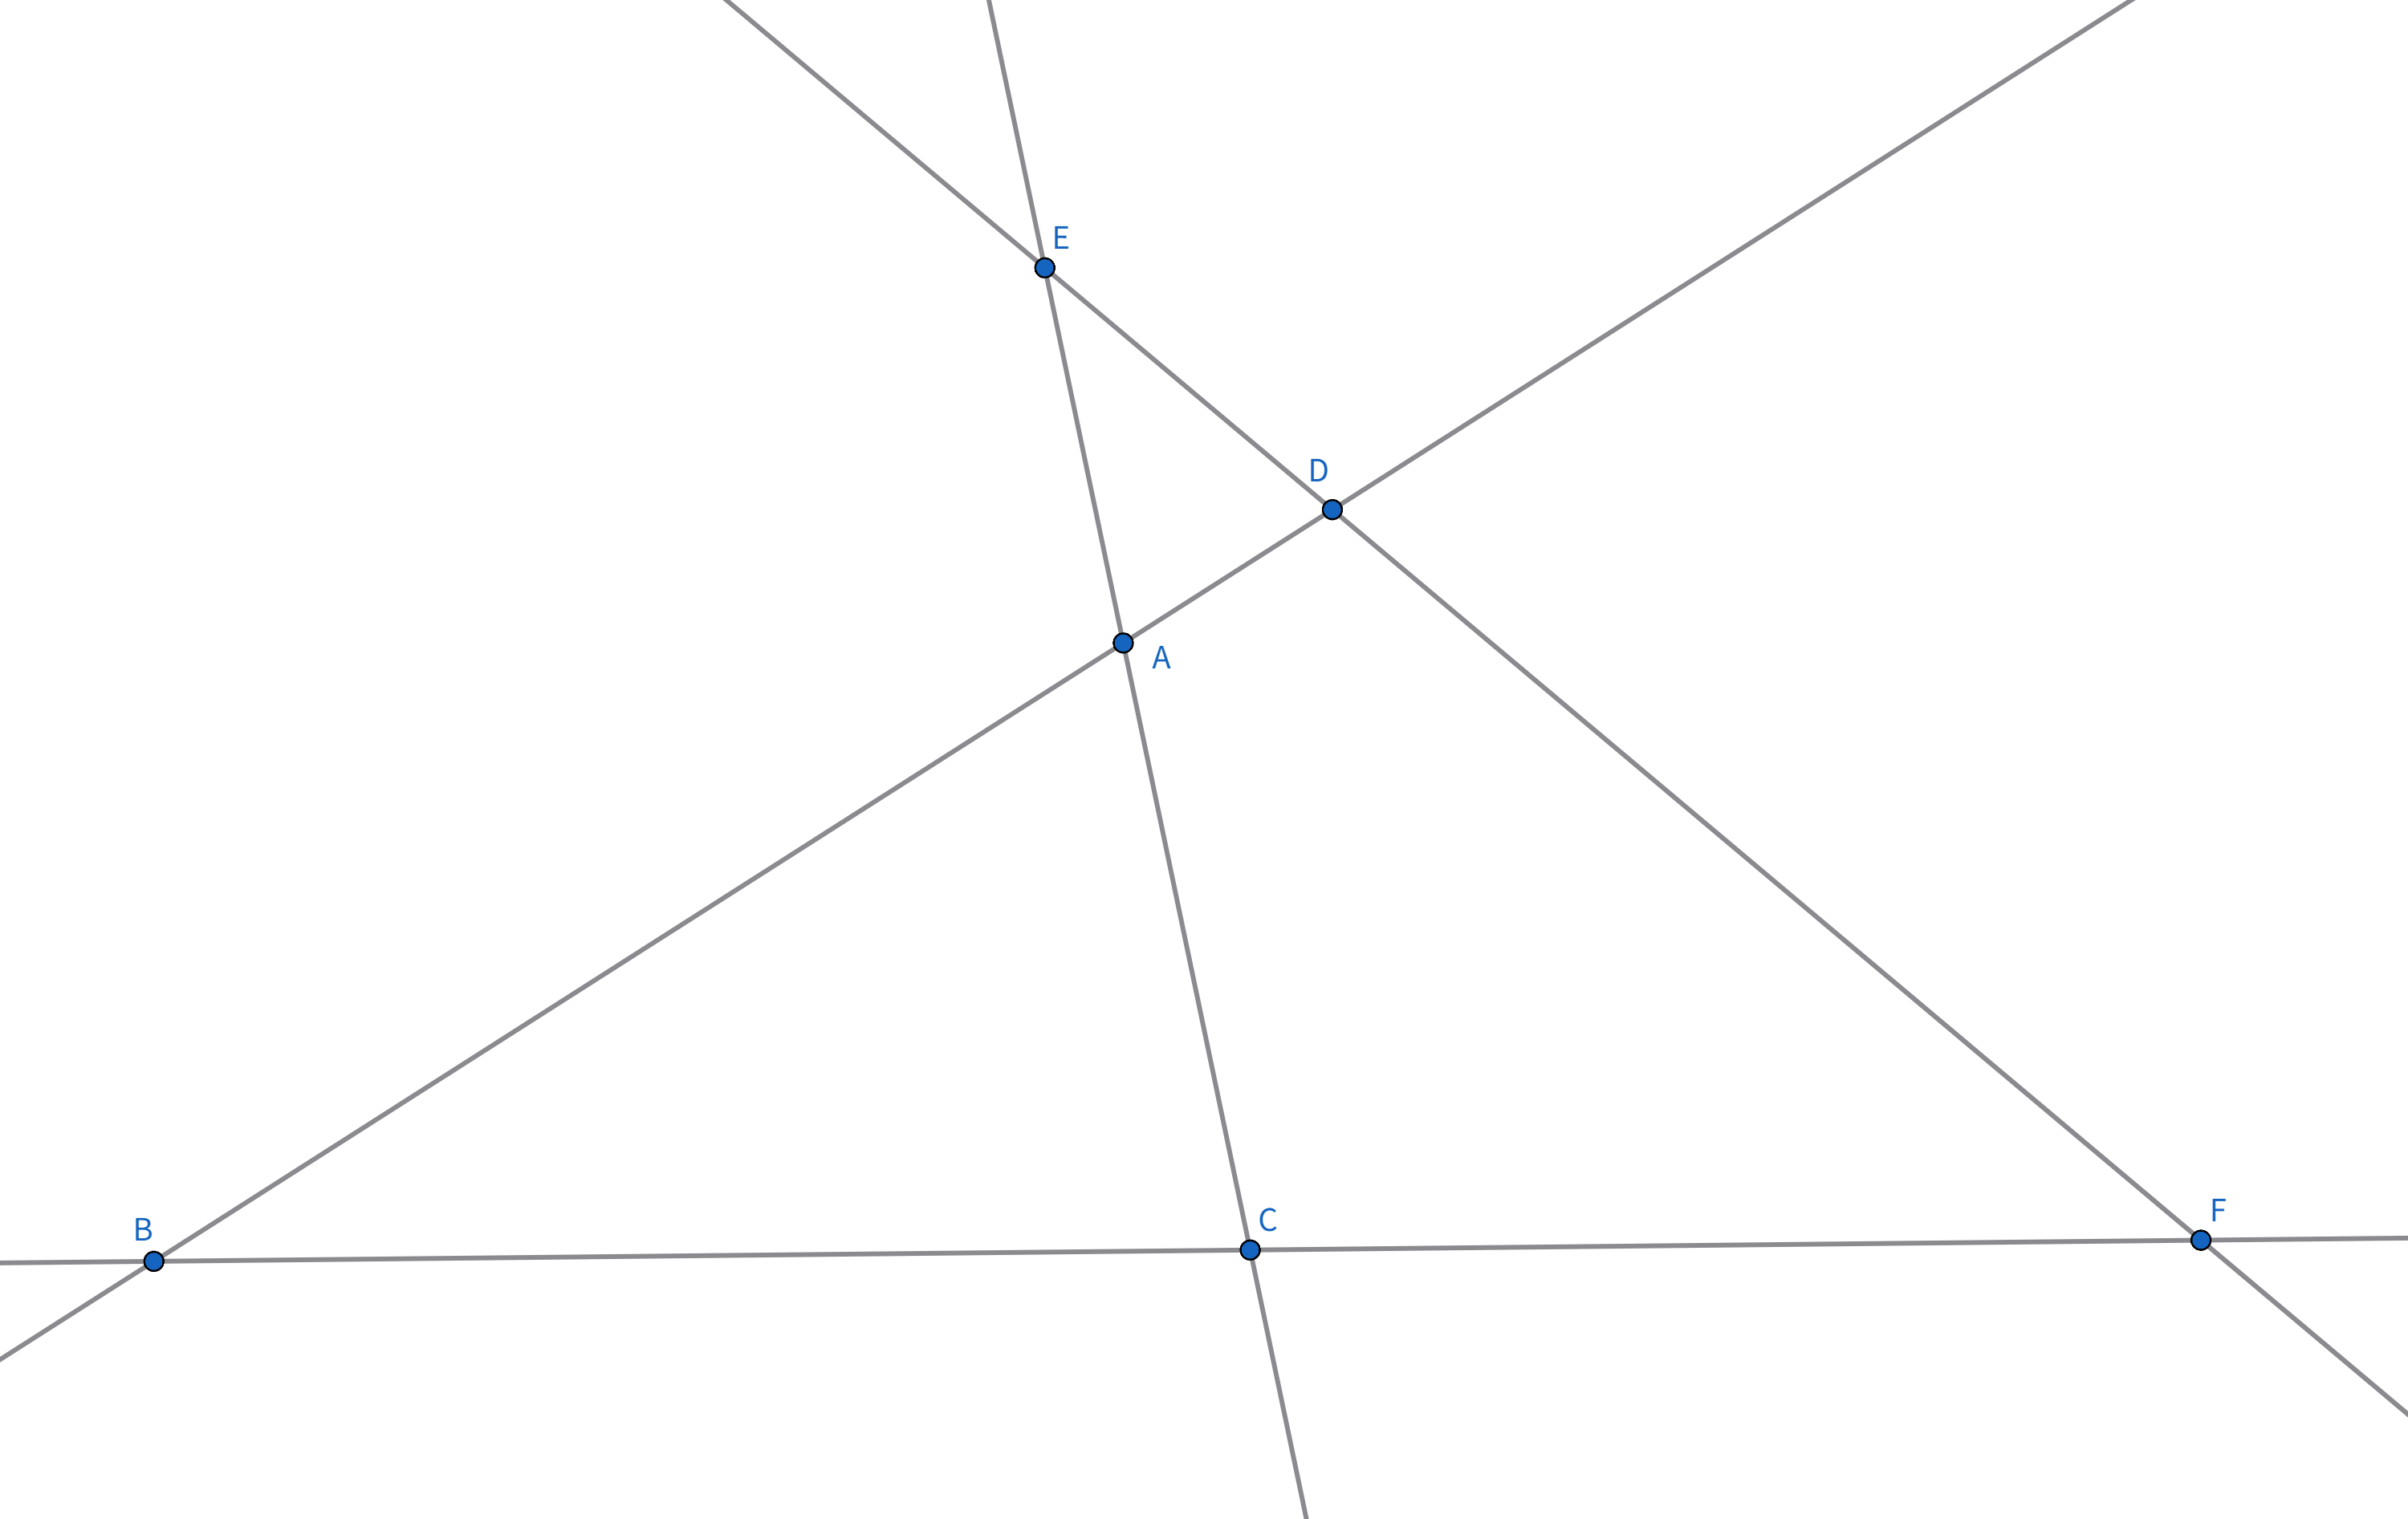
\includegraphics[width=\linewidth]{figures/menelaus (1).png}
    % \caption{情形2}
    \end{minipage}
\end{figure}


\begin{theorem}[梅涅劳斯(Menelaus)逆定理]
如果 $X 、 Y 、 Z$ 中有偶数个点在 $\triangle A B C$ 的三边上,且点 $X 、 Y 、 Z$ 分别为 $\triangle A B C$ 的三边 $B C 、 C A 、 A B$ 所在直线上的点,满足 
$$\frac{A Z}{Z B} \cdot \frac{B X}{X C} \cdot \frac{C Y}{Y A}=1,$$
则 $X 、 Y 、 Z$ 三点共线.
\end{theorem}



\begin{figure}[htbp]
    \centering
    \hfill % 添加一些水平间距
    \begin{minipage}[t]{0.45\textwidth}
        \centering
        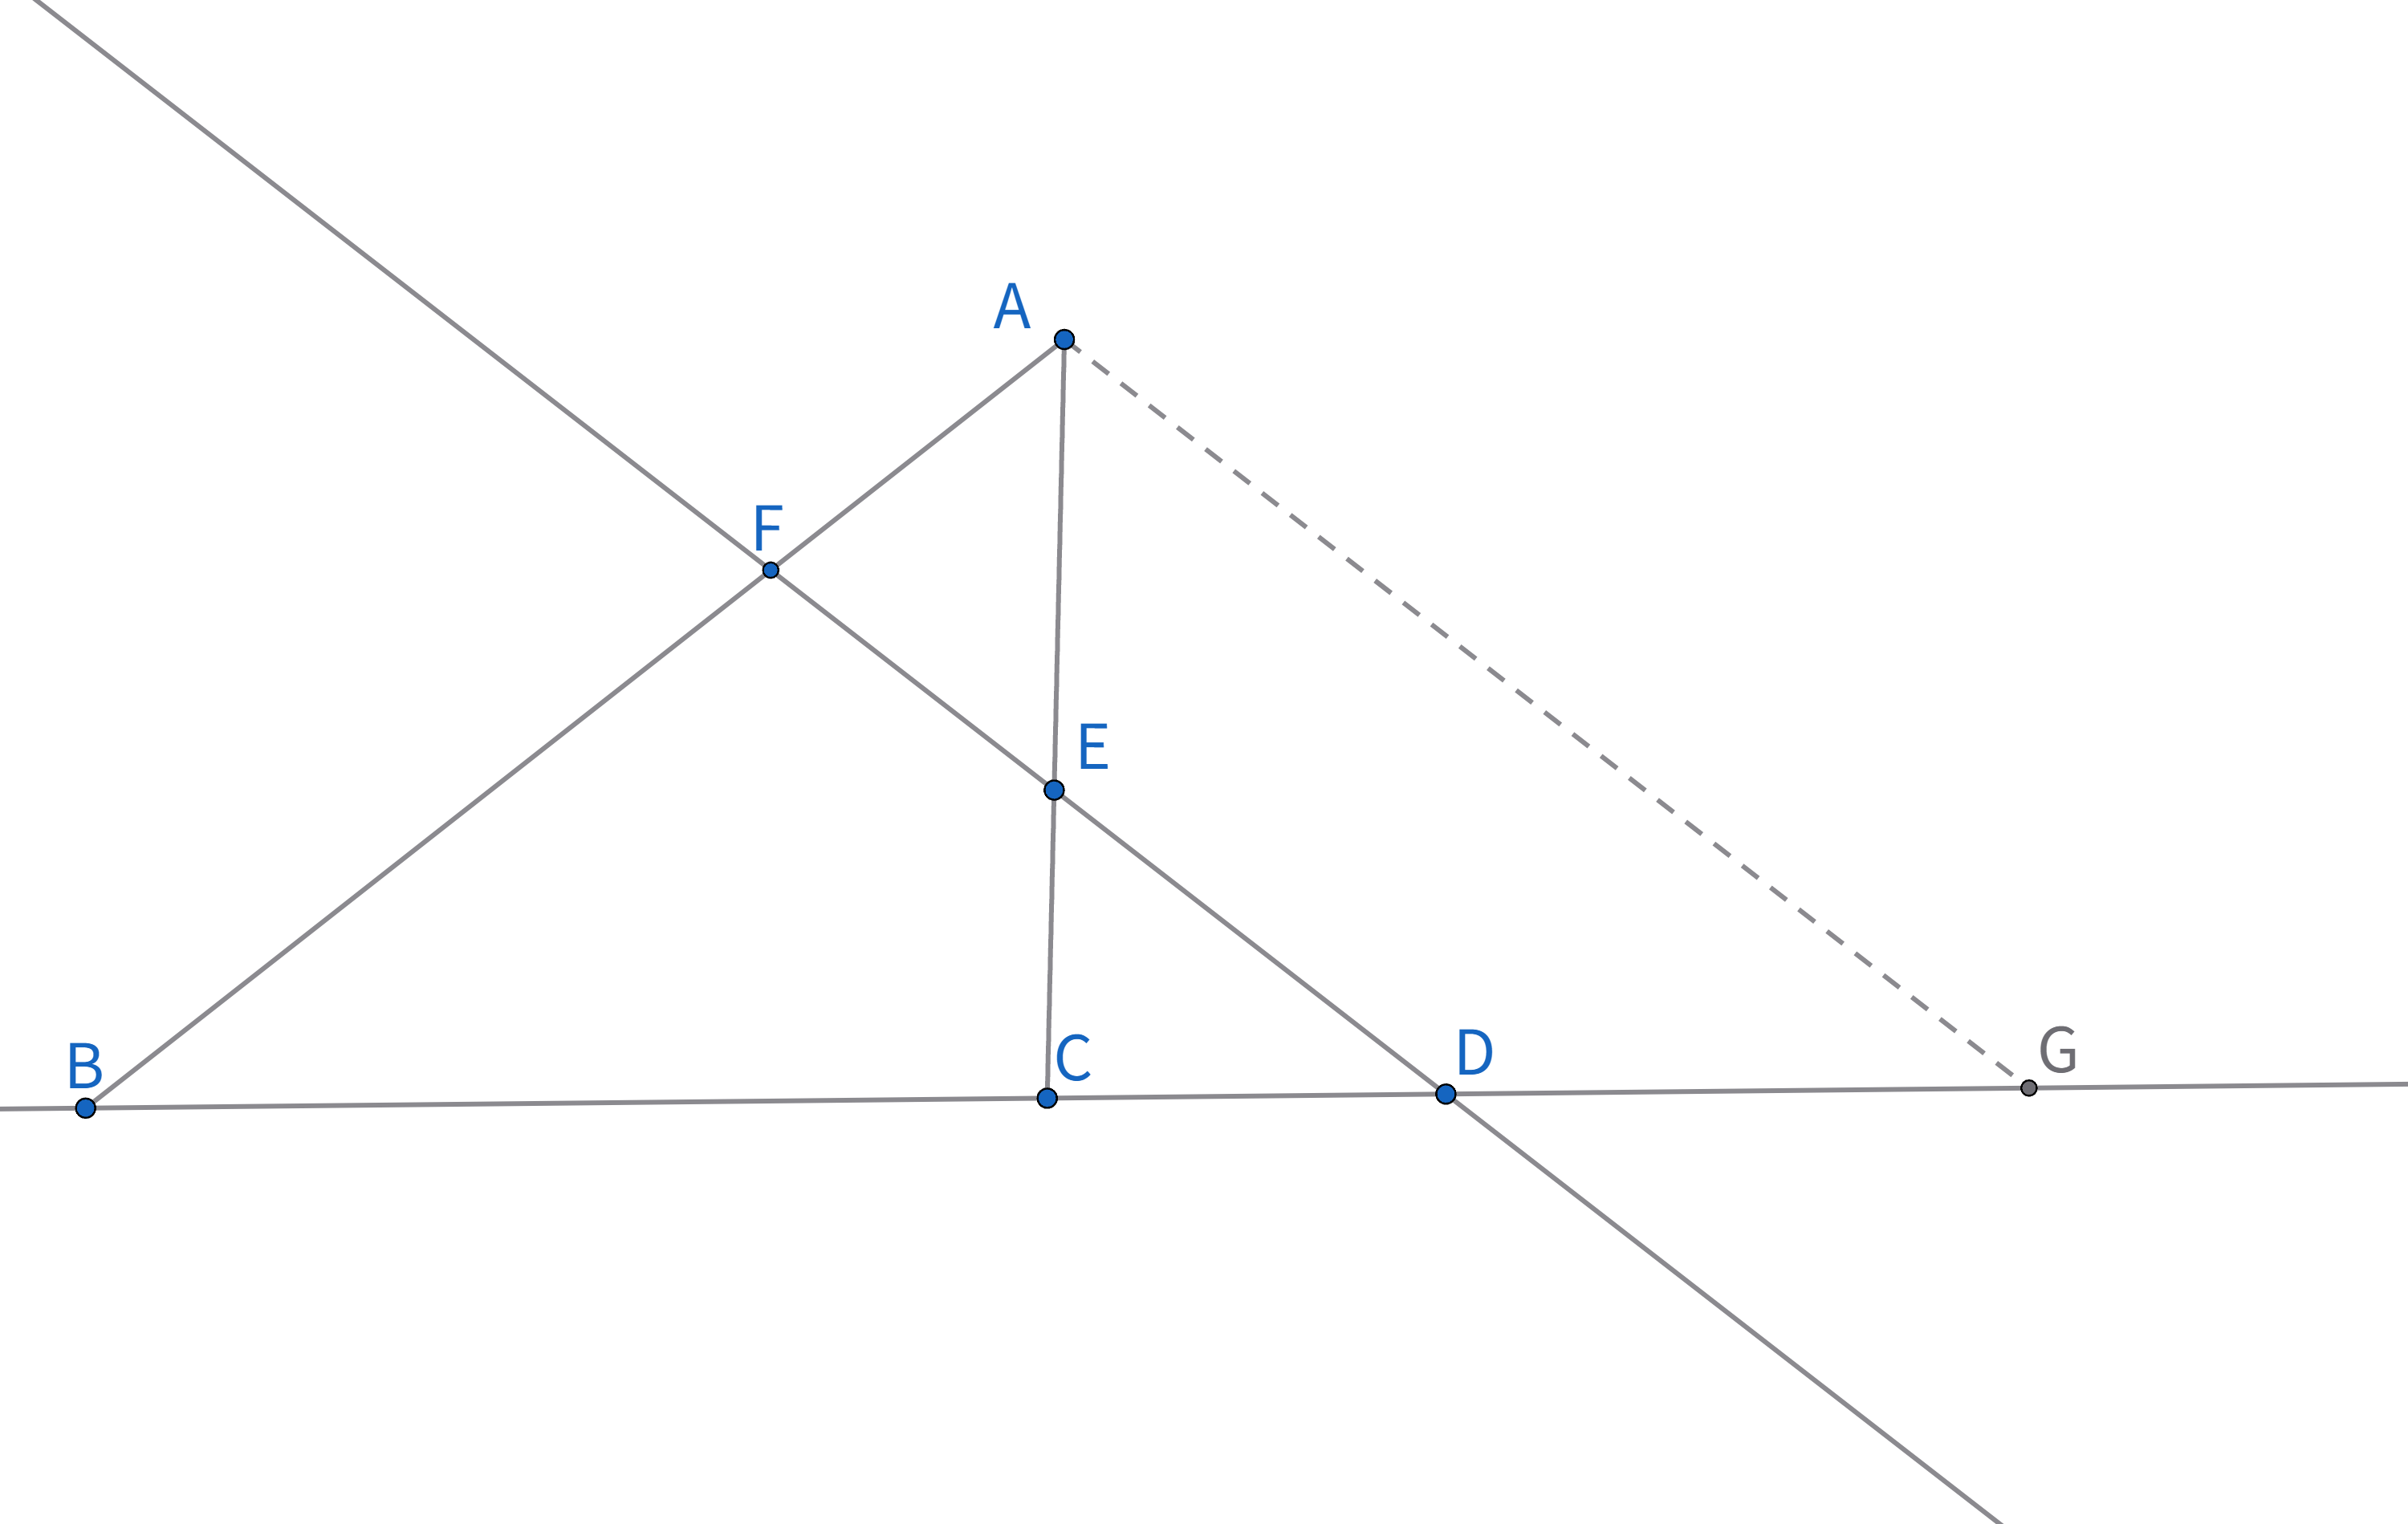
\includegraphics[width=\linewidth]{figures/menelaus辅助线1.png}
    \end{minipage}
    \hfill % 添加一些水平间距
    \begin{minipage}[t]{0.45\textwidth}
    \centering
    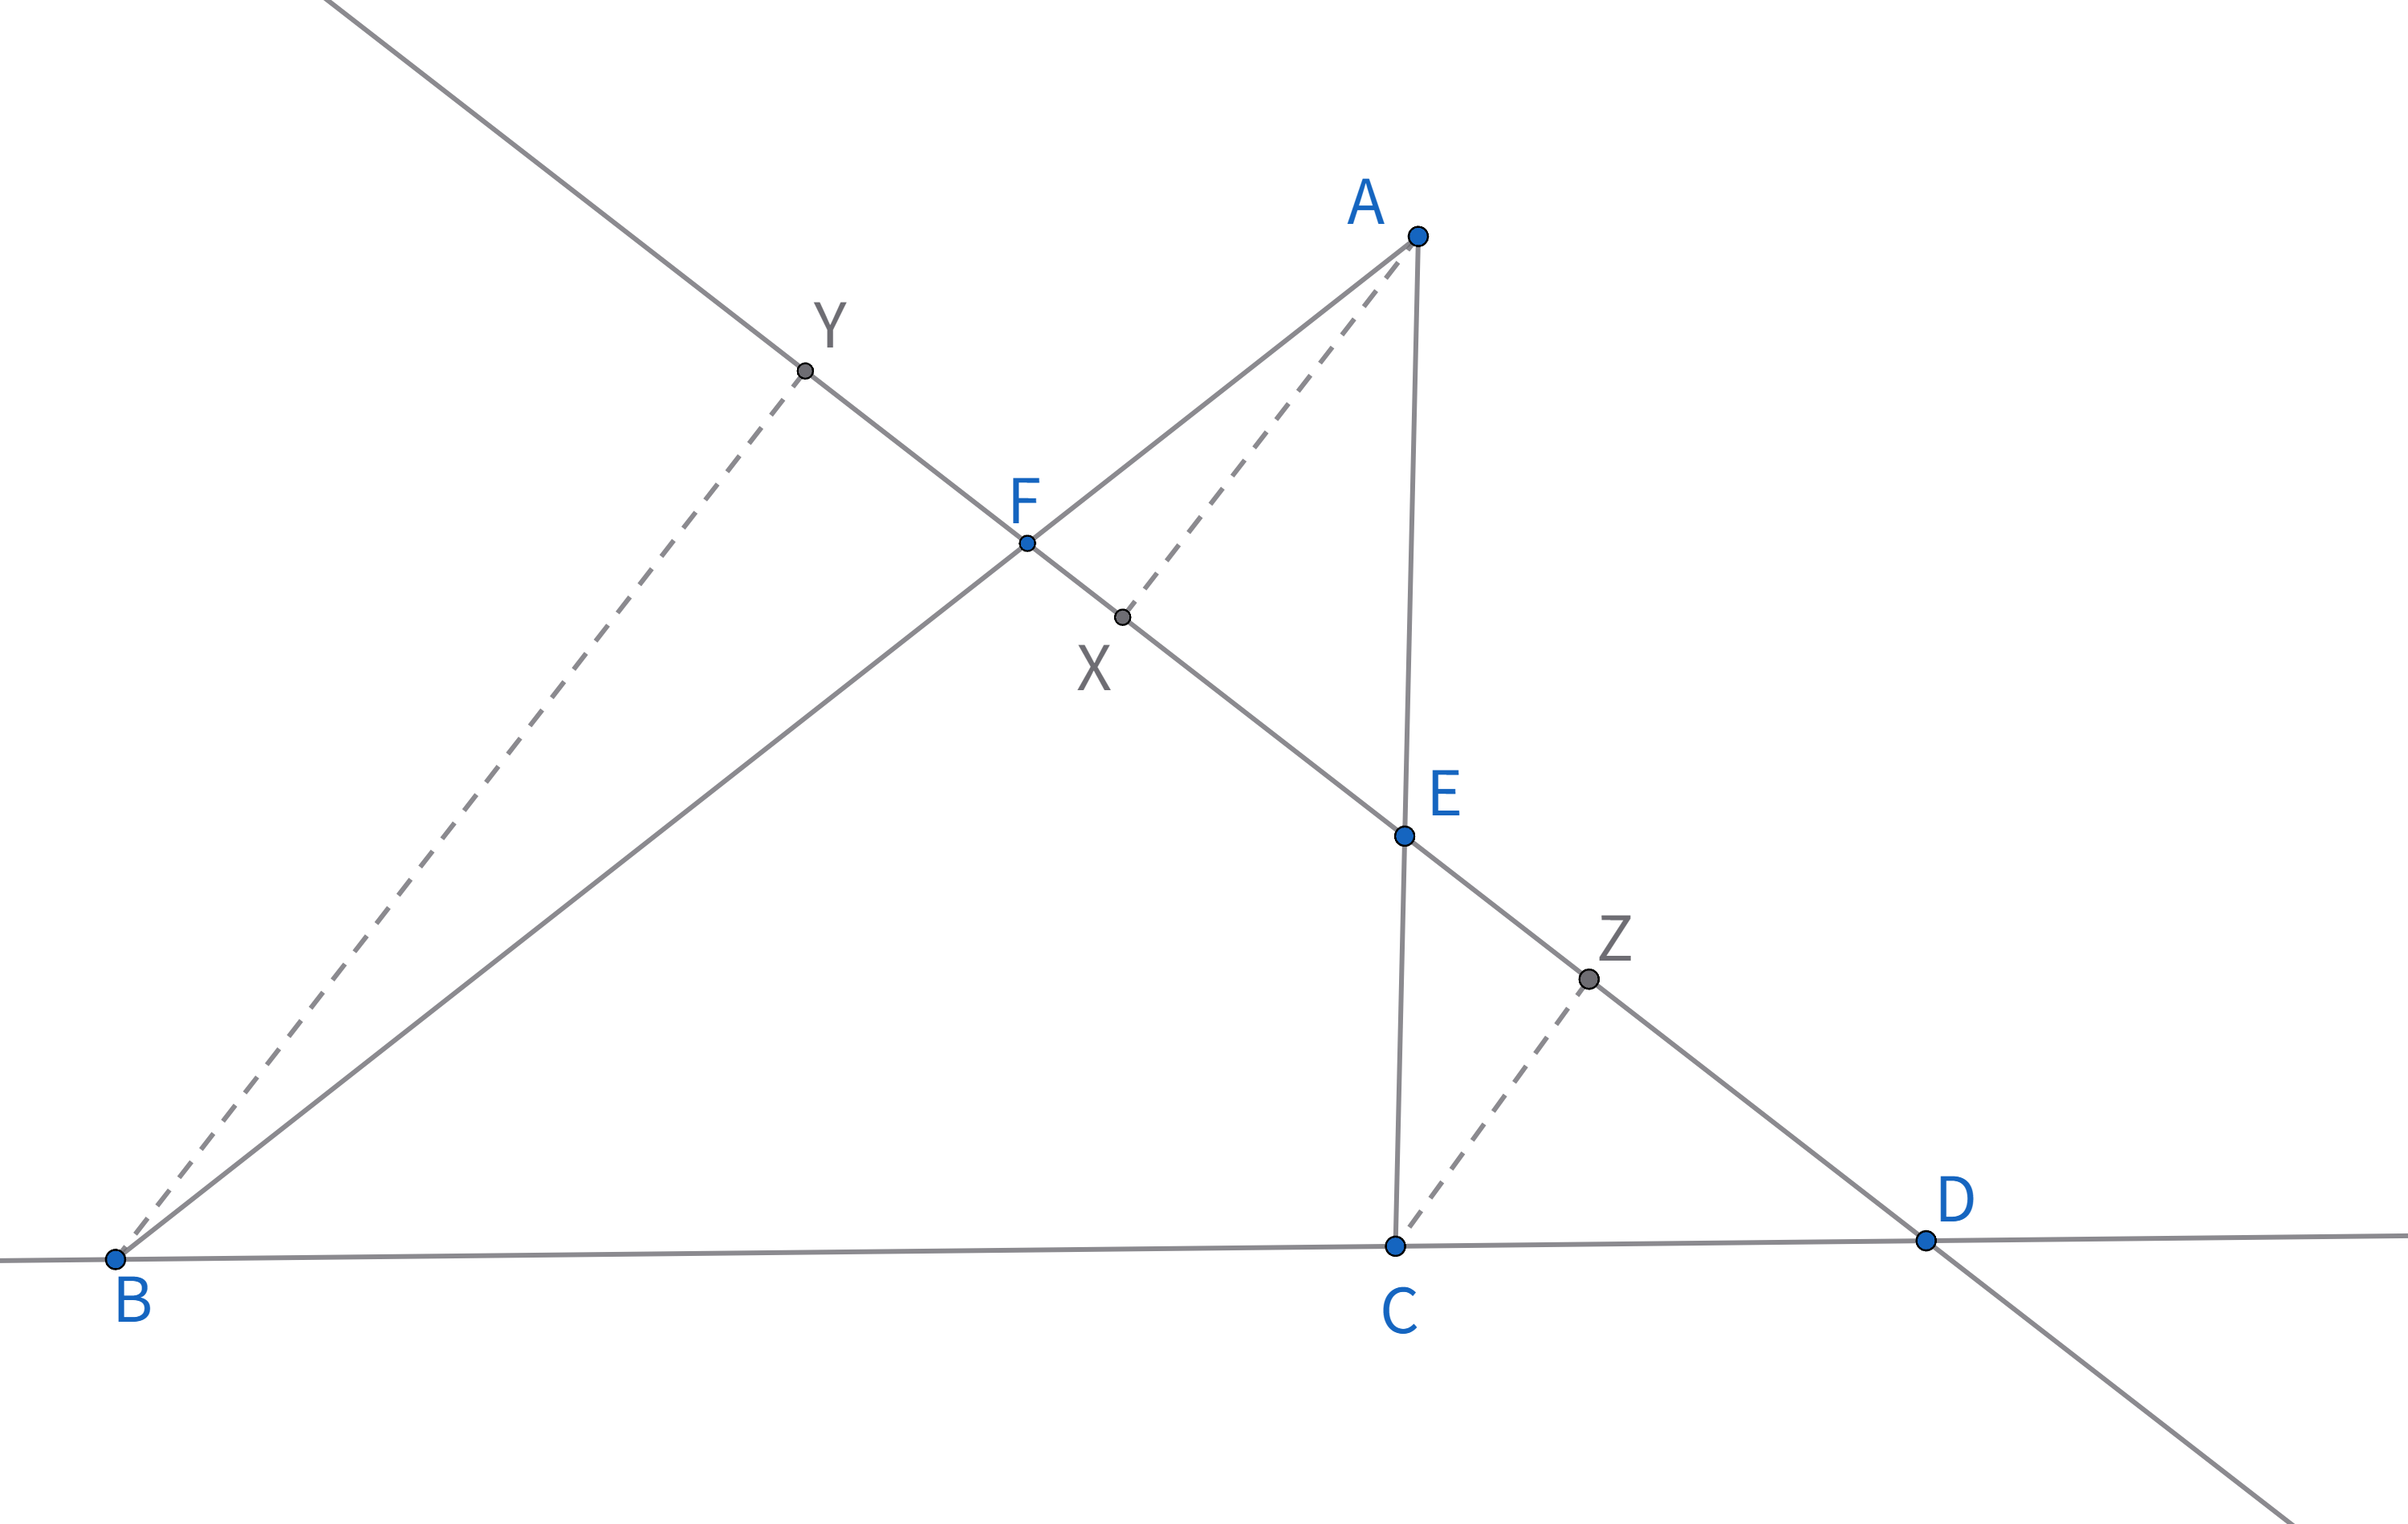
\includegraphics[width=\linewidth]{figures/menelaus辅助线2.png}
    \end{minipage}
\end{figure}

\begin{remark}
    梅涅劳斯定理中的恒等式可以按照顶点-截点-顶点的顺序记忆。
    
    例如对$\triangle ABC$首先确定三边顺序AB、BC、AC,然后确定各个边上的截点X、Y、Z,与各边顶点连接起来就得到了(AX-XB)-(BY-YC)-(CZ-ZA)。

    截线XYZ可以交于三边的延长线。

    正定理多用于获得截线段比值关系,逆定理多用于证明三点共线问题。
\end{remark}
%---------------------------------------------------
\newpage 
\subsection{塞瓦定理}
\begin{theorem}[塞瓦(Ceva)定理]
    已知平面上 $\triangle A B C$ 和点 $P$( $P$ 不在 $\triangle A B C$ 三边上),直线 $A P 、 B P 、 C P$ 分别与直线 $B C 、 C A 、 A B$ 交于点 $X 、 Y 、 Z$ ,则 
    $$\frac{A Z}{Z B} \cdot \frac{B X}{X C} \cdot \frac{C Y}{Y A}=1.$$
\end{theorem}


\begin{figure}[htbp]
    \centering
    \hfill % 添加一些水平间距
    \begin{minipage}[t]{0.3\textwidth}
        \centering
        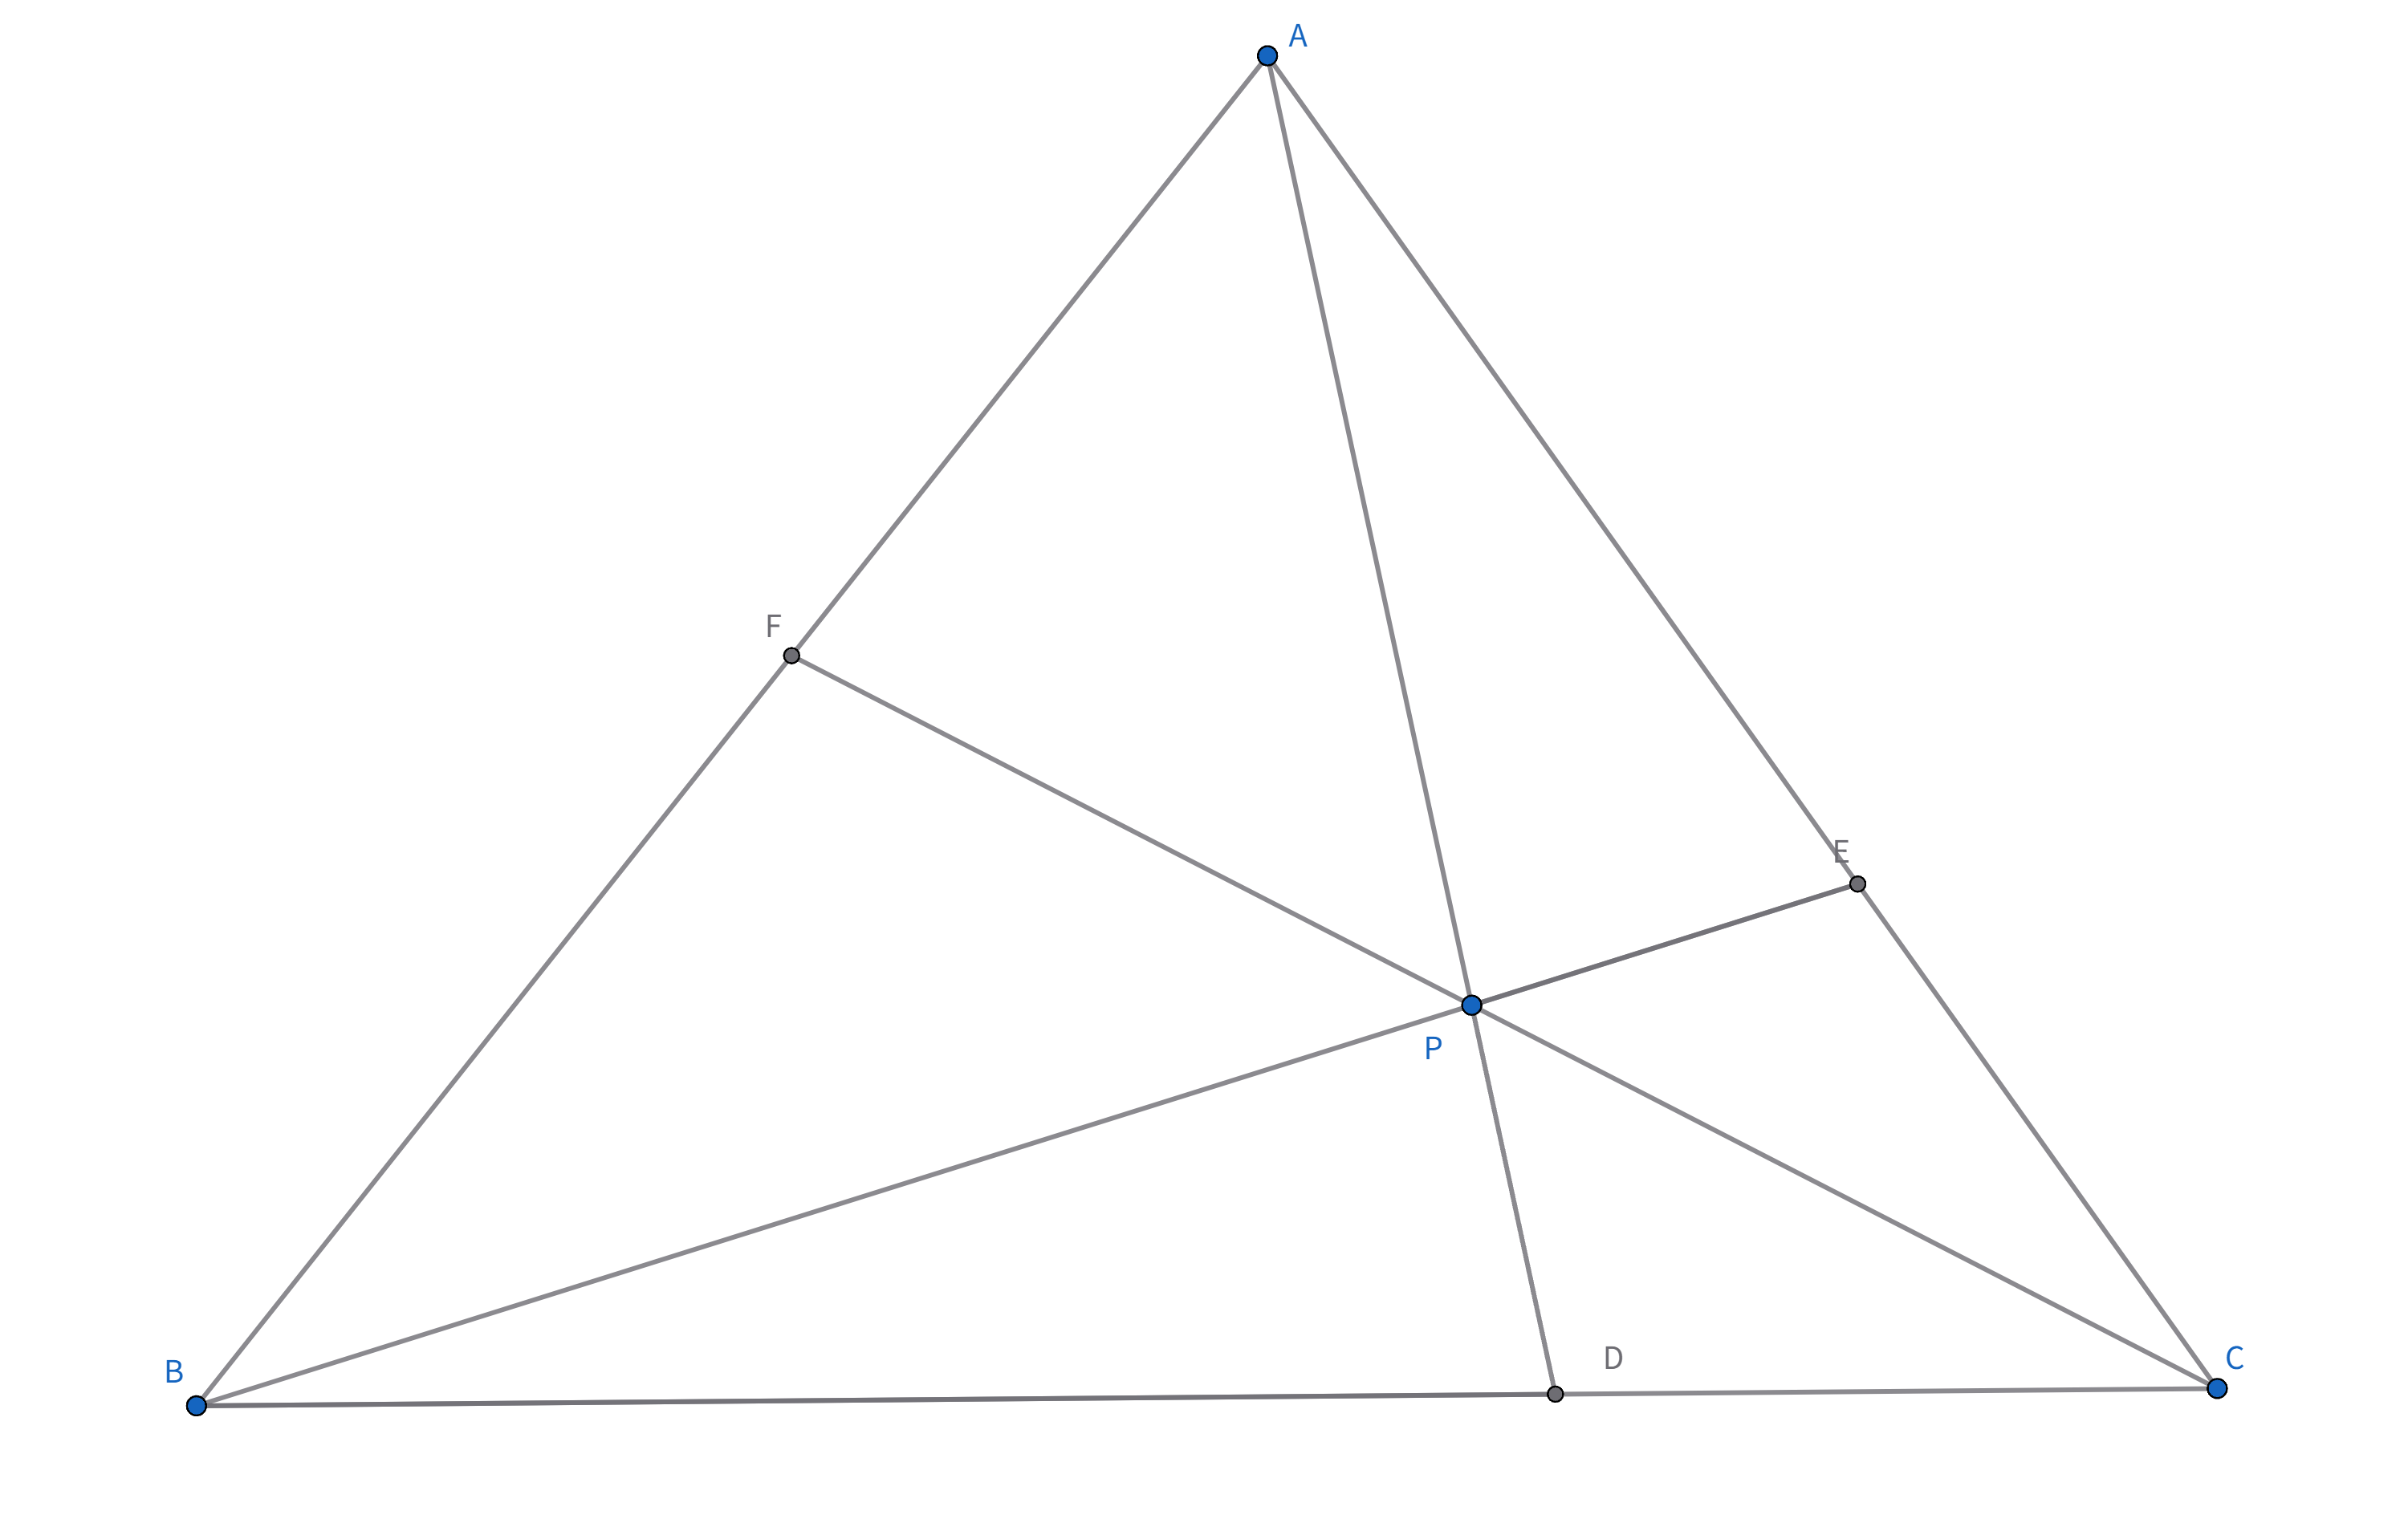
\includegraphics[width=\linewidth]{figures/ceva (2).png}
        \caption{情形1}
    \end{minipage}
    \hfill % 添加一些水平间距
    \begin{minipage}[t]{0.3\textwidth}
    \centering
    \includegraphics[width=\linewidth]{figures/ceva.png}
    \caption{情形2}
    \end{minipage}
        \hfill % 添加一些水平间距
    \begin{minipage}[t]{0.3\textwidth}
    \centering
    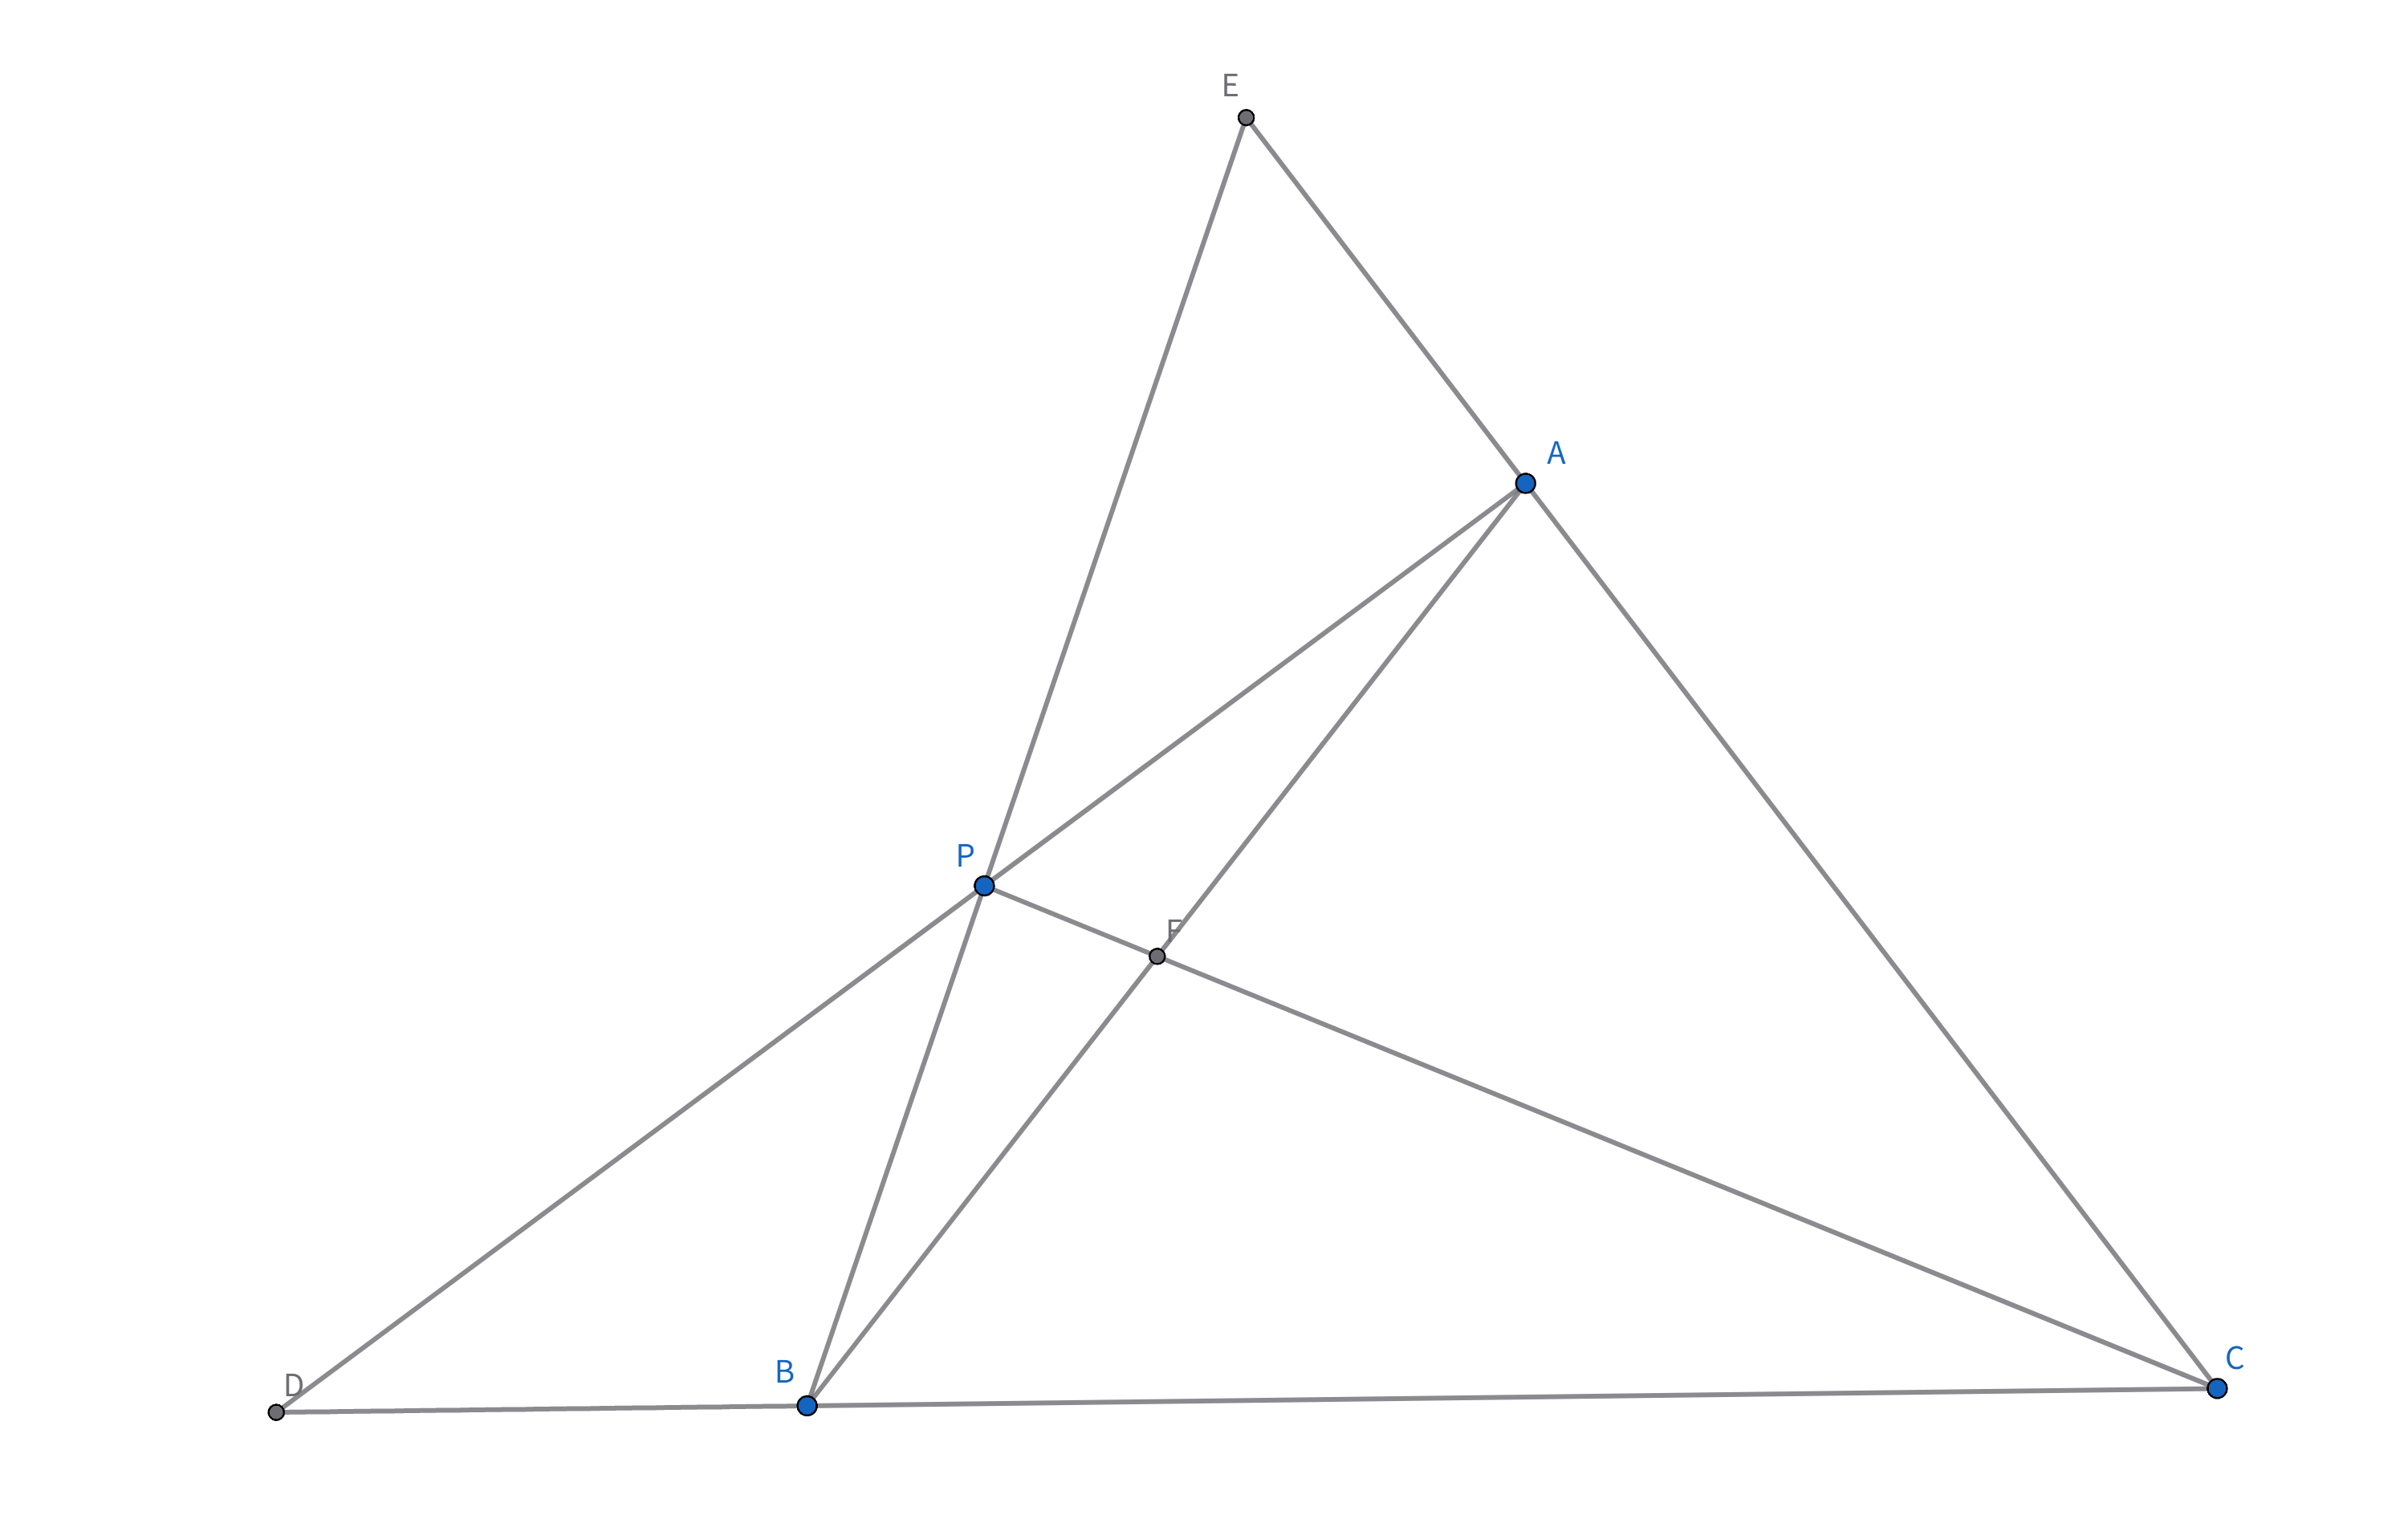
\includegraphics[width=\linewidth]{figures/ceva (1).png}
    \caption{情形3}
    \end{minipage}
\end{figure}


\begin{theorem}[塞瓦(Ceva)逆定理]
如果 $X 、 Y 、 Z$ 中有奇数个点在 $\triangle A B C$ 的三边上,且点 $X 、 Y 、$ $Z$ 分别为 $\triangle A B C$ 的三边 $B C 、 C A 、 A B$ 所在直线上的点,满足 
$$\frac{A Z}{Z B} \cdot \frac{B X}{X C} \cdot \frac{C Y}{Y A}=1,$$
则 $A X 、 B Y 、 C Z$ 三条直线交于一点或彼此平行.
\end{theorem}


\begin{figure}[htbp]
    \centering
    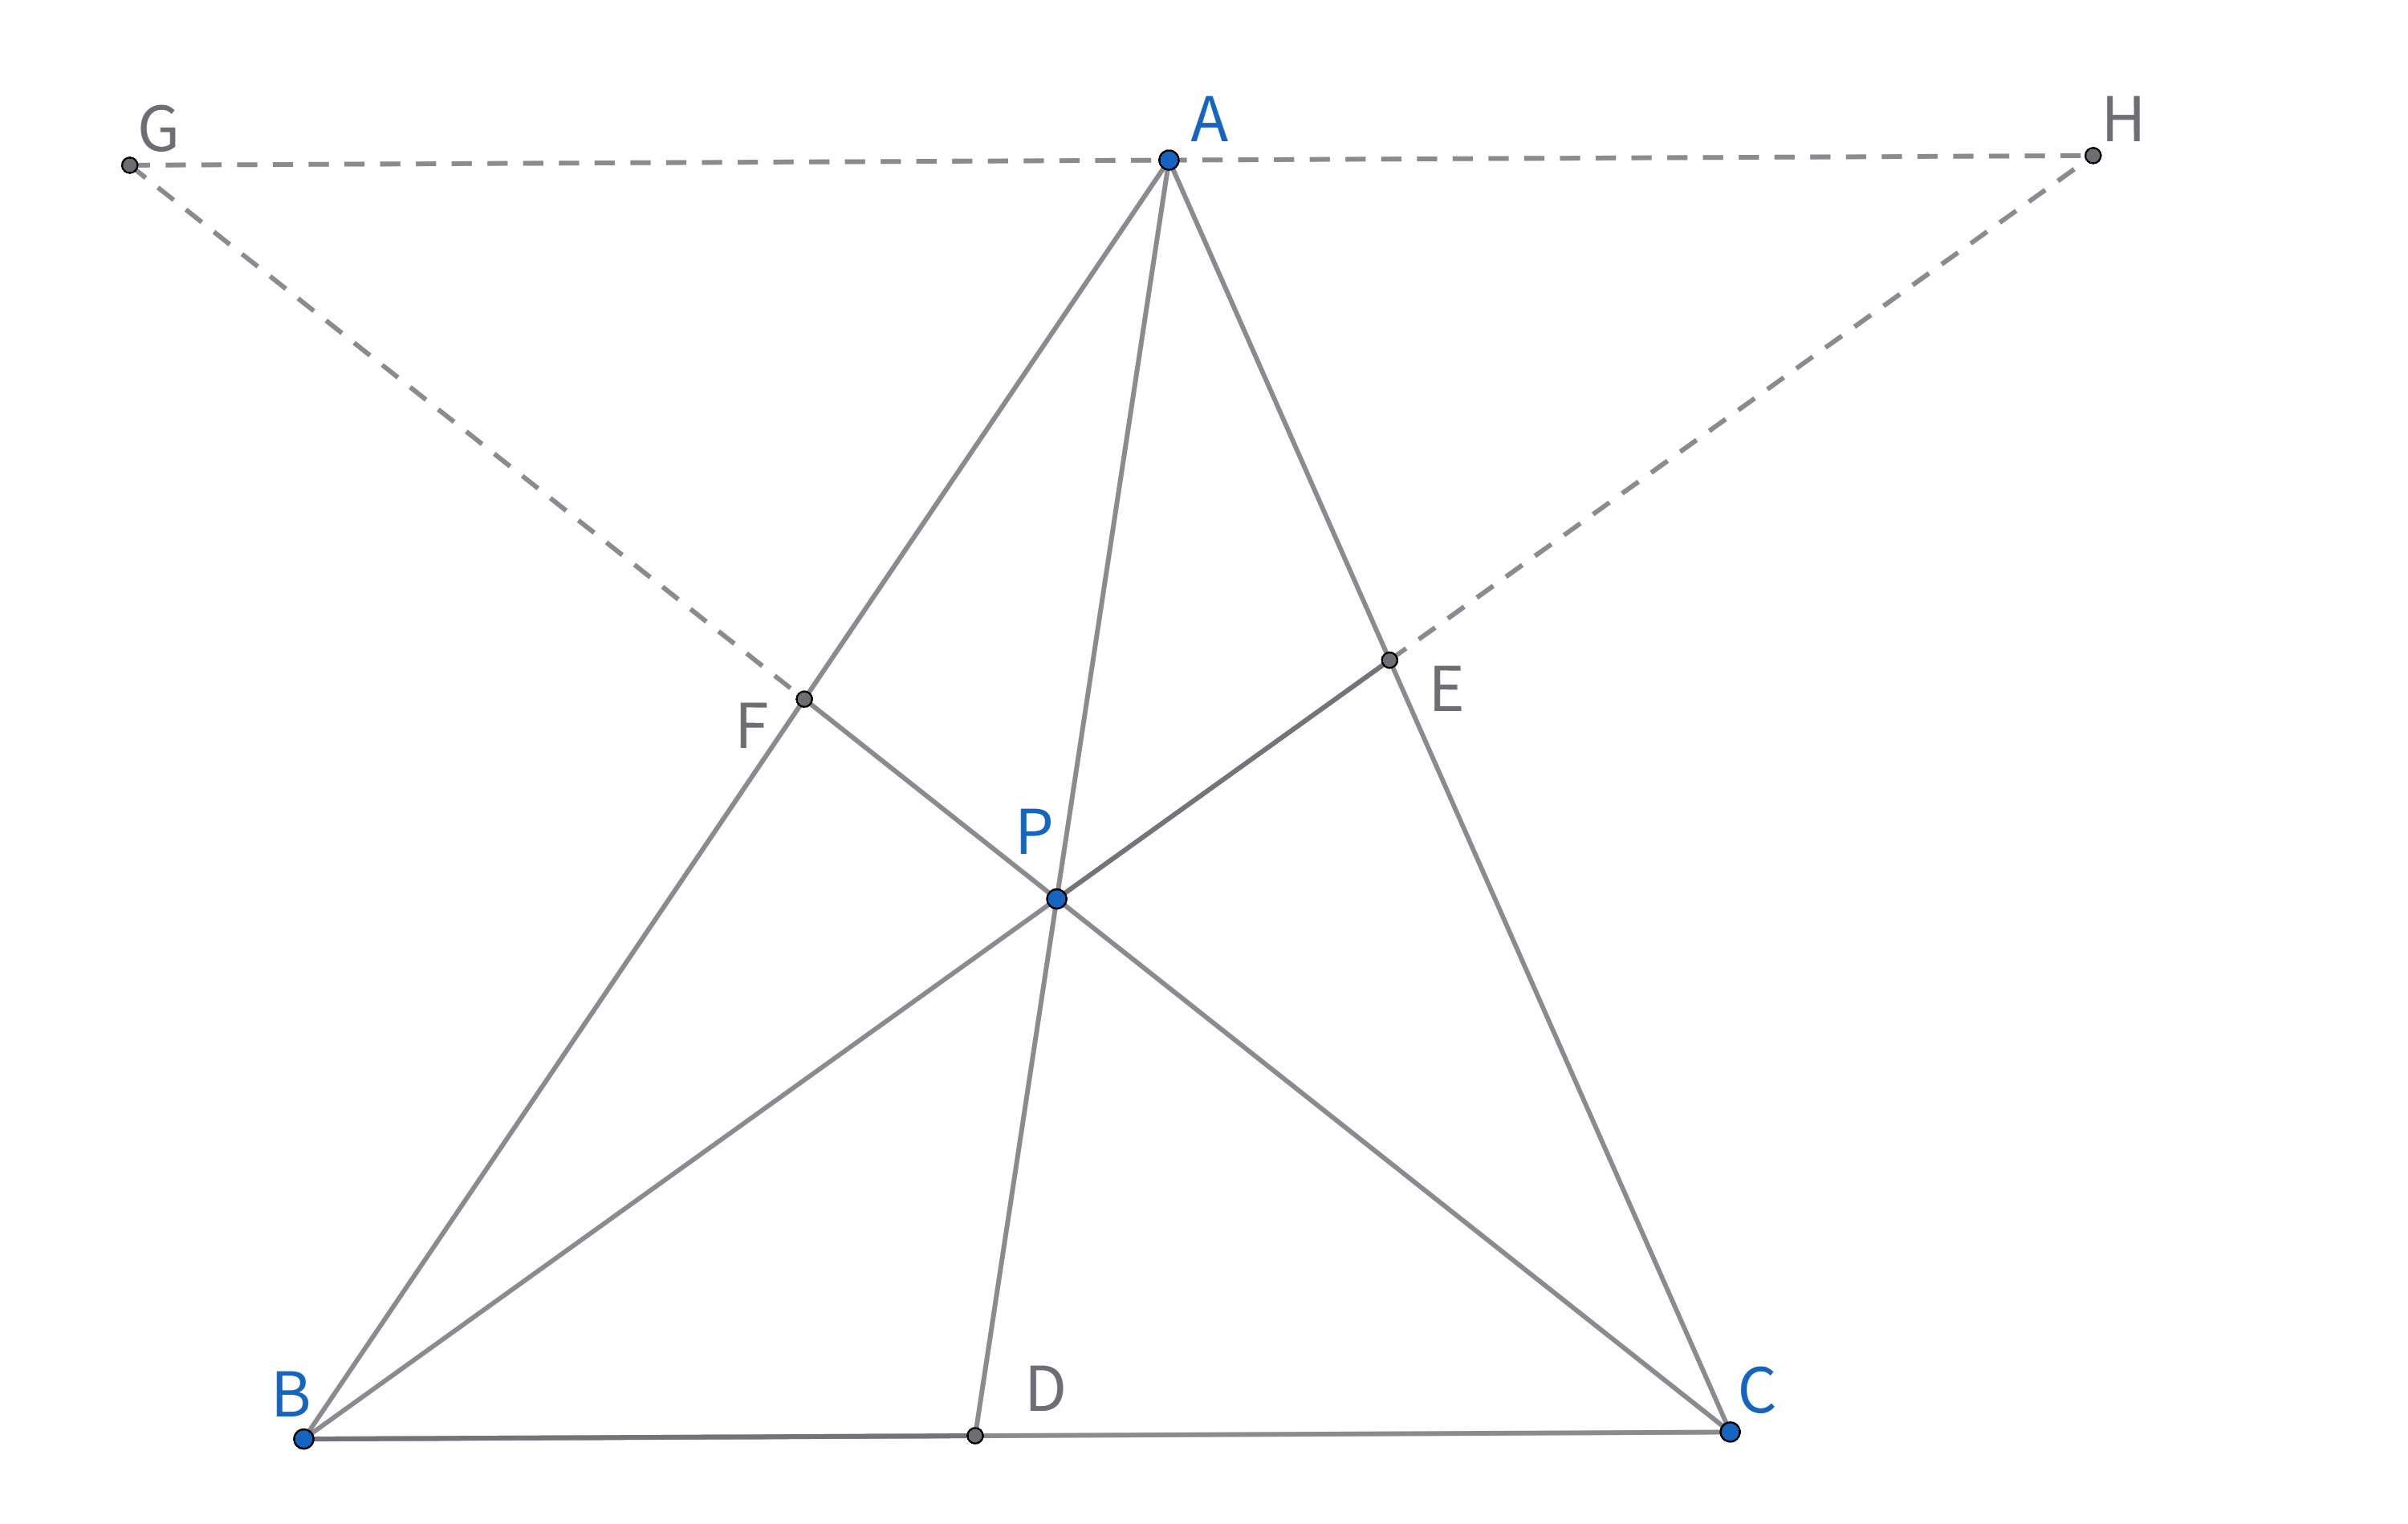
\includegraphics[width=0.6\linewidth]{figures/ceva辅助线.png}
\end{figure}
\begin{remark}
    塞瓦定理与梅涅劳斯定理的记忆方法类似,都是按照顶点-截点-顶点的顺序。

    塞瓦定理中点P可以不在$\triangle ABC$形内。
    
    P为无穷原点时,BE、AD、CF三线平行,等式依然成立。

    
\end{remark}


\begin{theorem}[角元形式赛瓦定理]
    已知平面上 $\triangle A B C$ 和点P( P不在$\triangle A B C$ 三边上)。设D、E、F分别是BC、CA、AB所在直线上的点。则AD、BE、CF三线共点等价于
    $$
    \frac{\sin \angle ABE}{\sin \angle EBC}
    \cdot 
    \frac{\sin \angle BCF}{\sin \angle FCA}
    \cdot 
    \frac{\sin \angle CAD}{\sin \angle DAB}
    =1
    $$
\end{theorem}


%---------------------------------------------------
\newpage 
\subsection{西姆松定理}
\begin{theorem}[西姆松(Simson)定理]
过$\triangle ABC$外接圆O上异于三角形顶点的任意一点P作三边所在直线的垂线,则三垂足共线,此线称为西姆松线(Simson line)。

西姆松定理的逆定理为:若一点P在$\triangle ABC$三边所在直线上的射影共线,则该点在此三角形的外接圆上。
\end{theorem}

\begin{figure}[htbp]
    \centering
    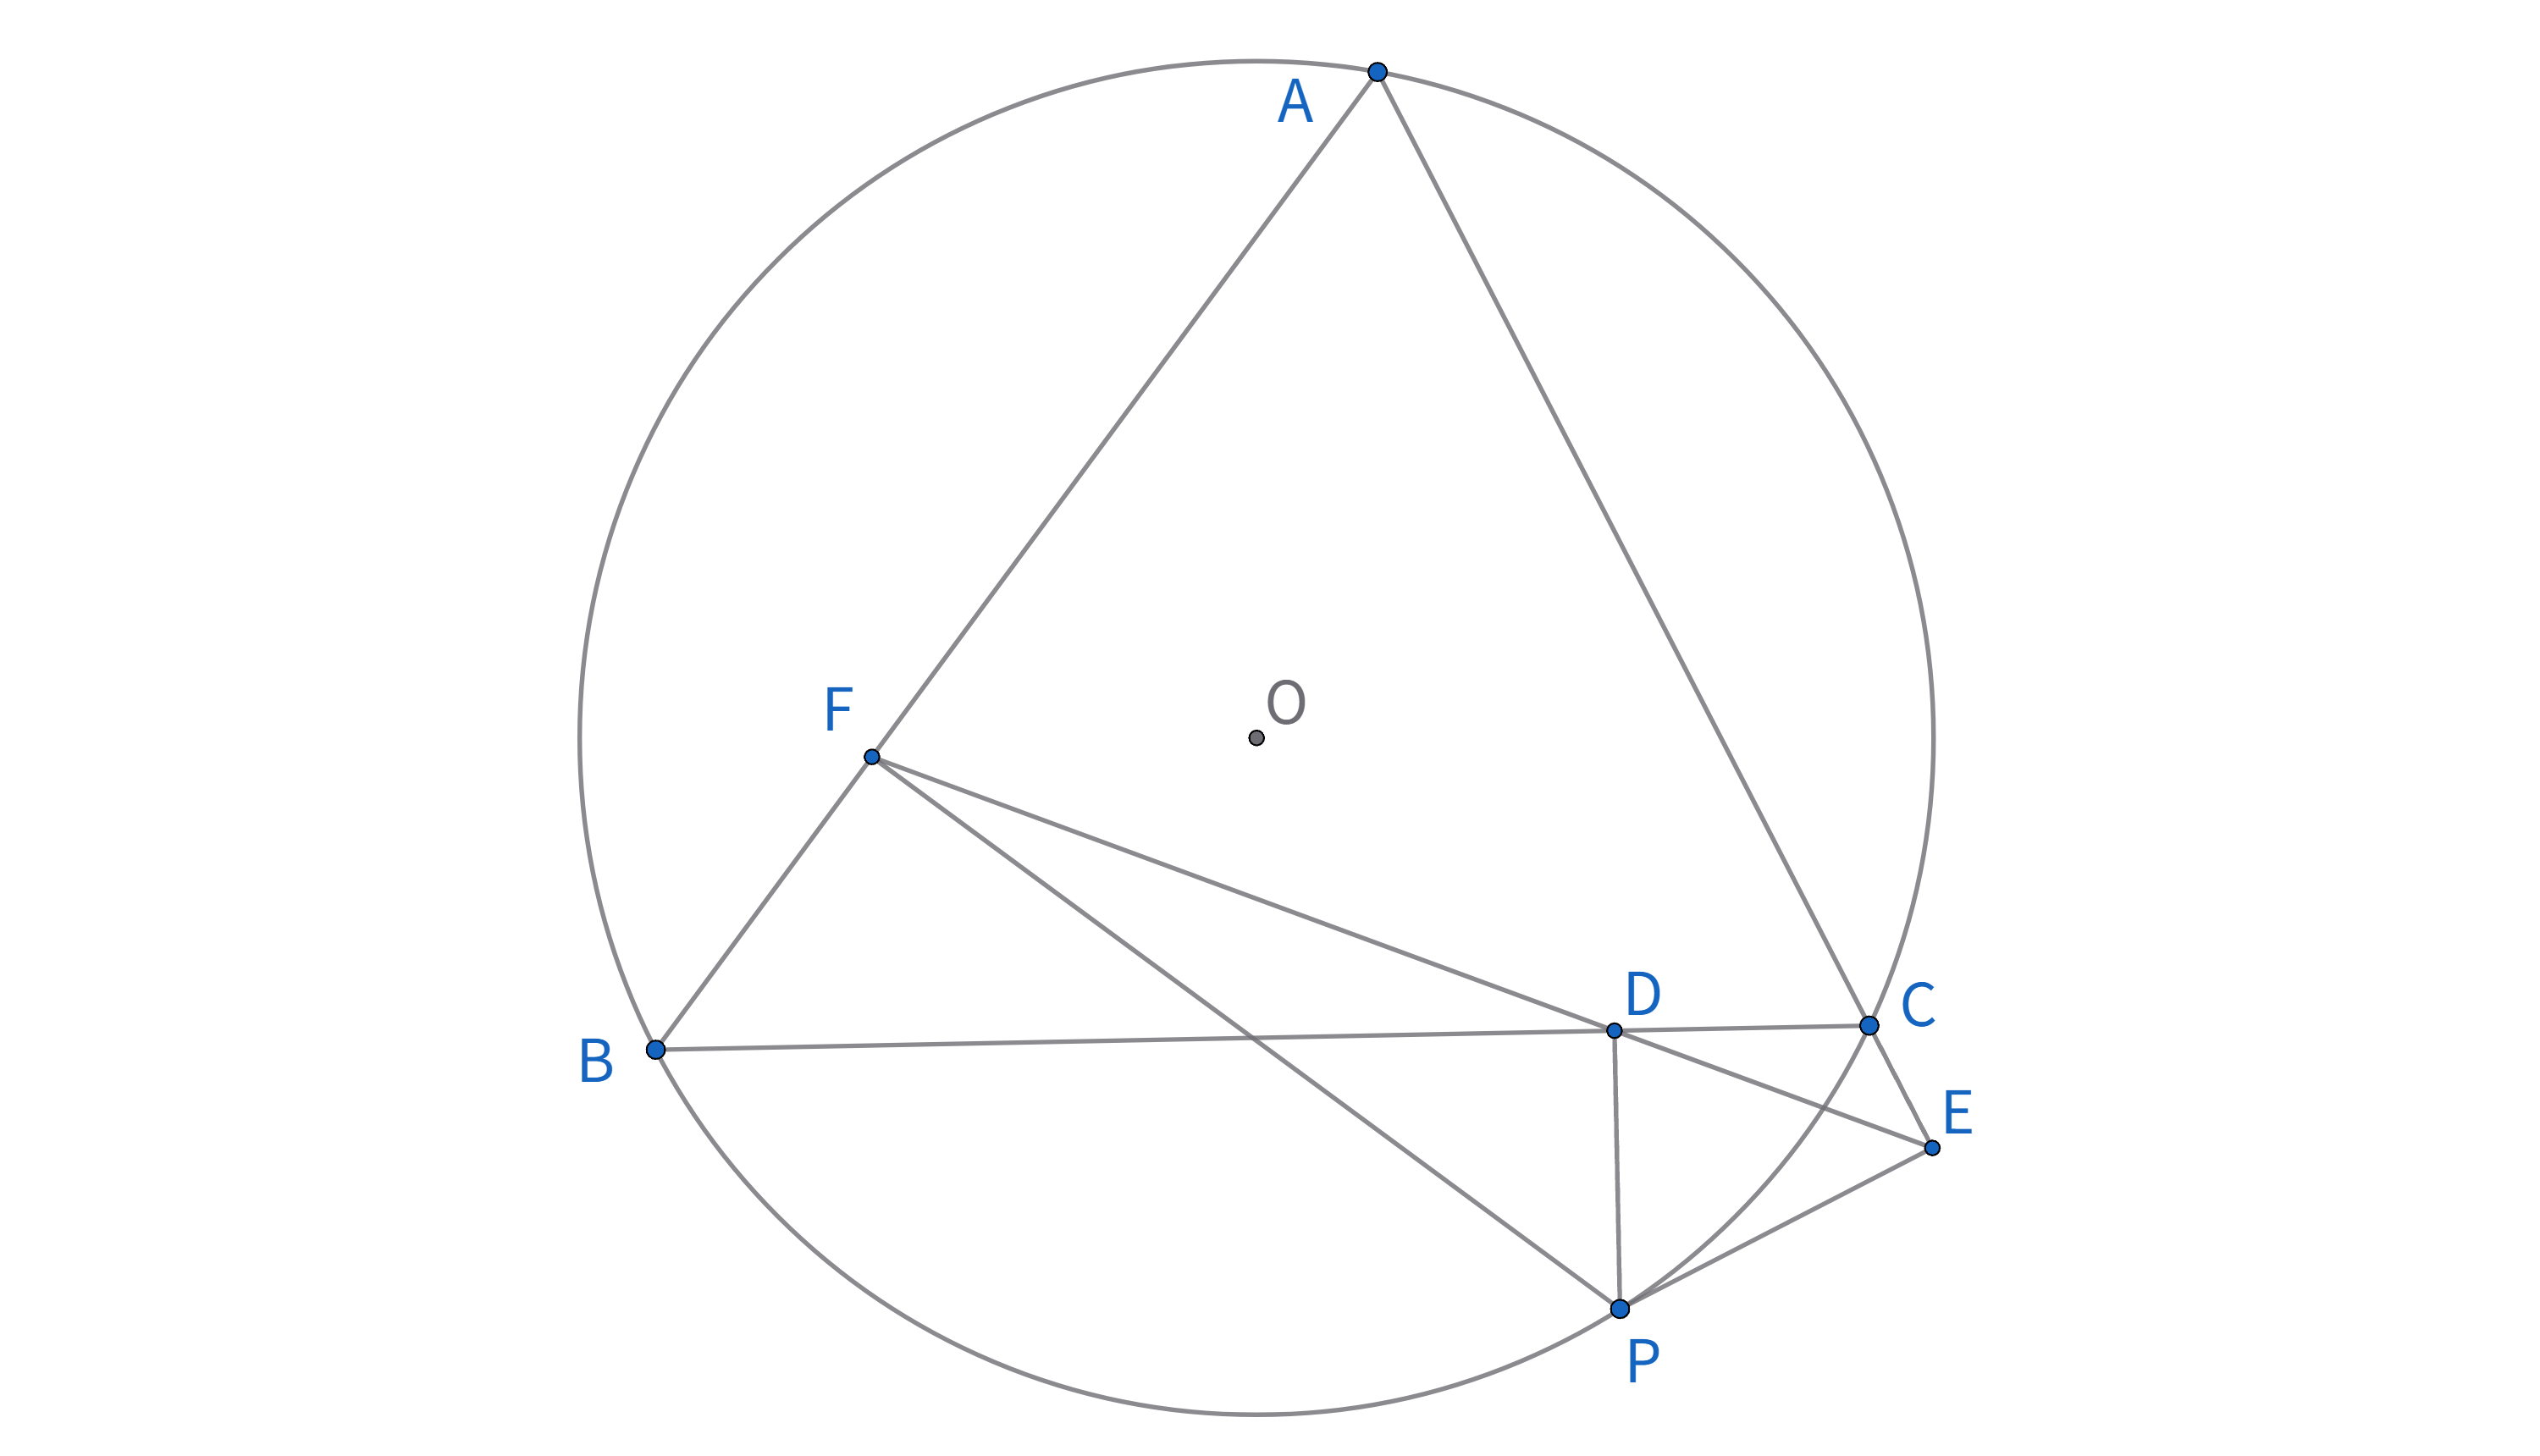
\includegraphics[width=\linewidth]{figures/西姆松线.png}
    \caption{西姆松线}
\end{figure}


%---------------------------------------------------
\newpage
\subsection{帕普斯定理}
\begin{theorem}[帕普斯(Pappus)定理]
直线l1上依次有点A、B、C,直线l2上依次有点D、E、F。
设AE、BD交于P,AF、DC交于Q,BF、EC交于R,则P、Q、R共线。
\end{theorem}
\begin{figure}[htbp]
    \centering
    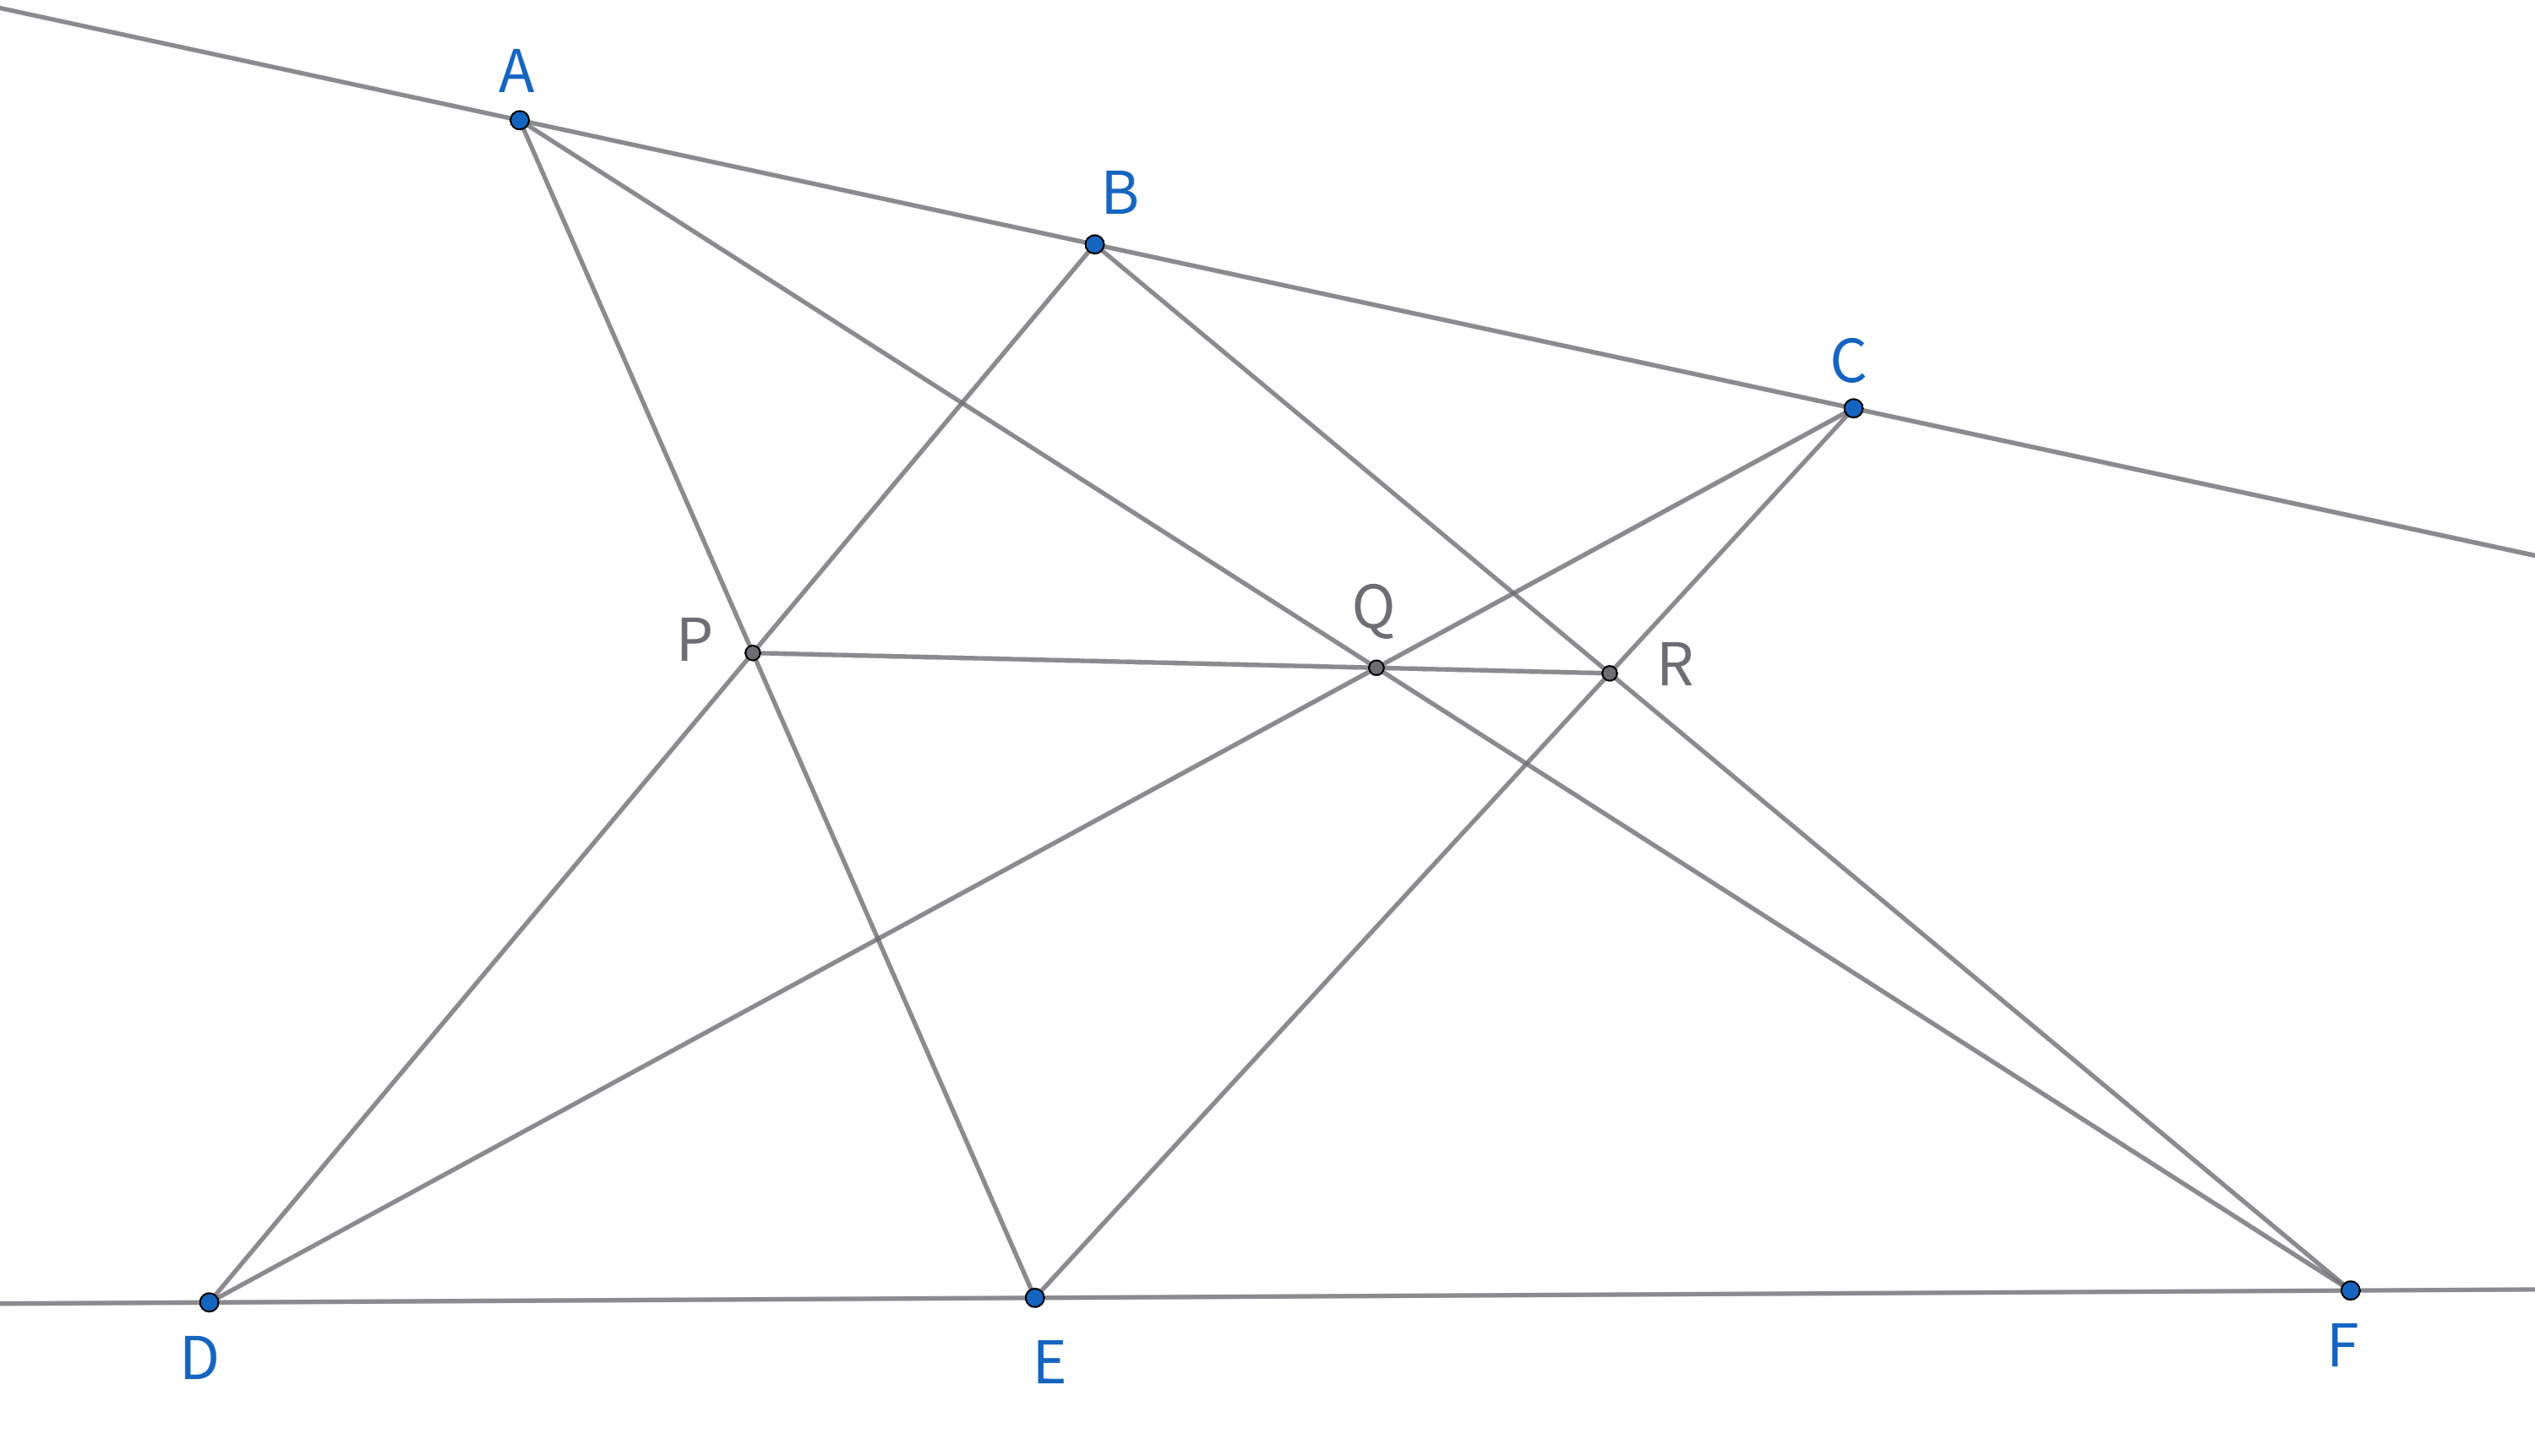
\includegraphics[width=\linewidth]{figures/帕普斯定理.png}
    \caption{帕普斯定理}
\end{figure}


%---------------------------------------------------
\newpage
\subsection{帕斯卡定理}
\begin{theorem}[帕斯卡(Pascal)定理]
设A、B、C、D、E、F为圆O上的点,
设AE、BD交于P,AF、DC交于Q,BF、EC交于R,则P、Q、R共线。
\end{theorem}
\begin{figure}[htbp]
    \centering
    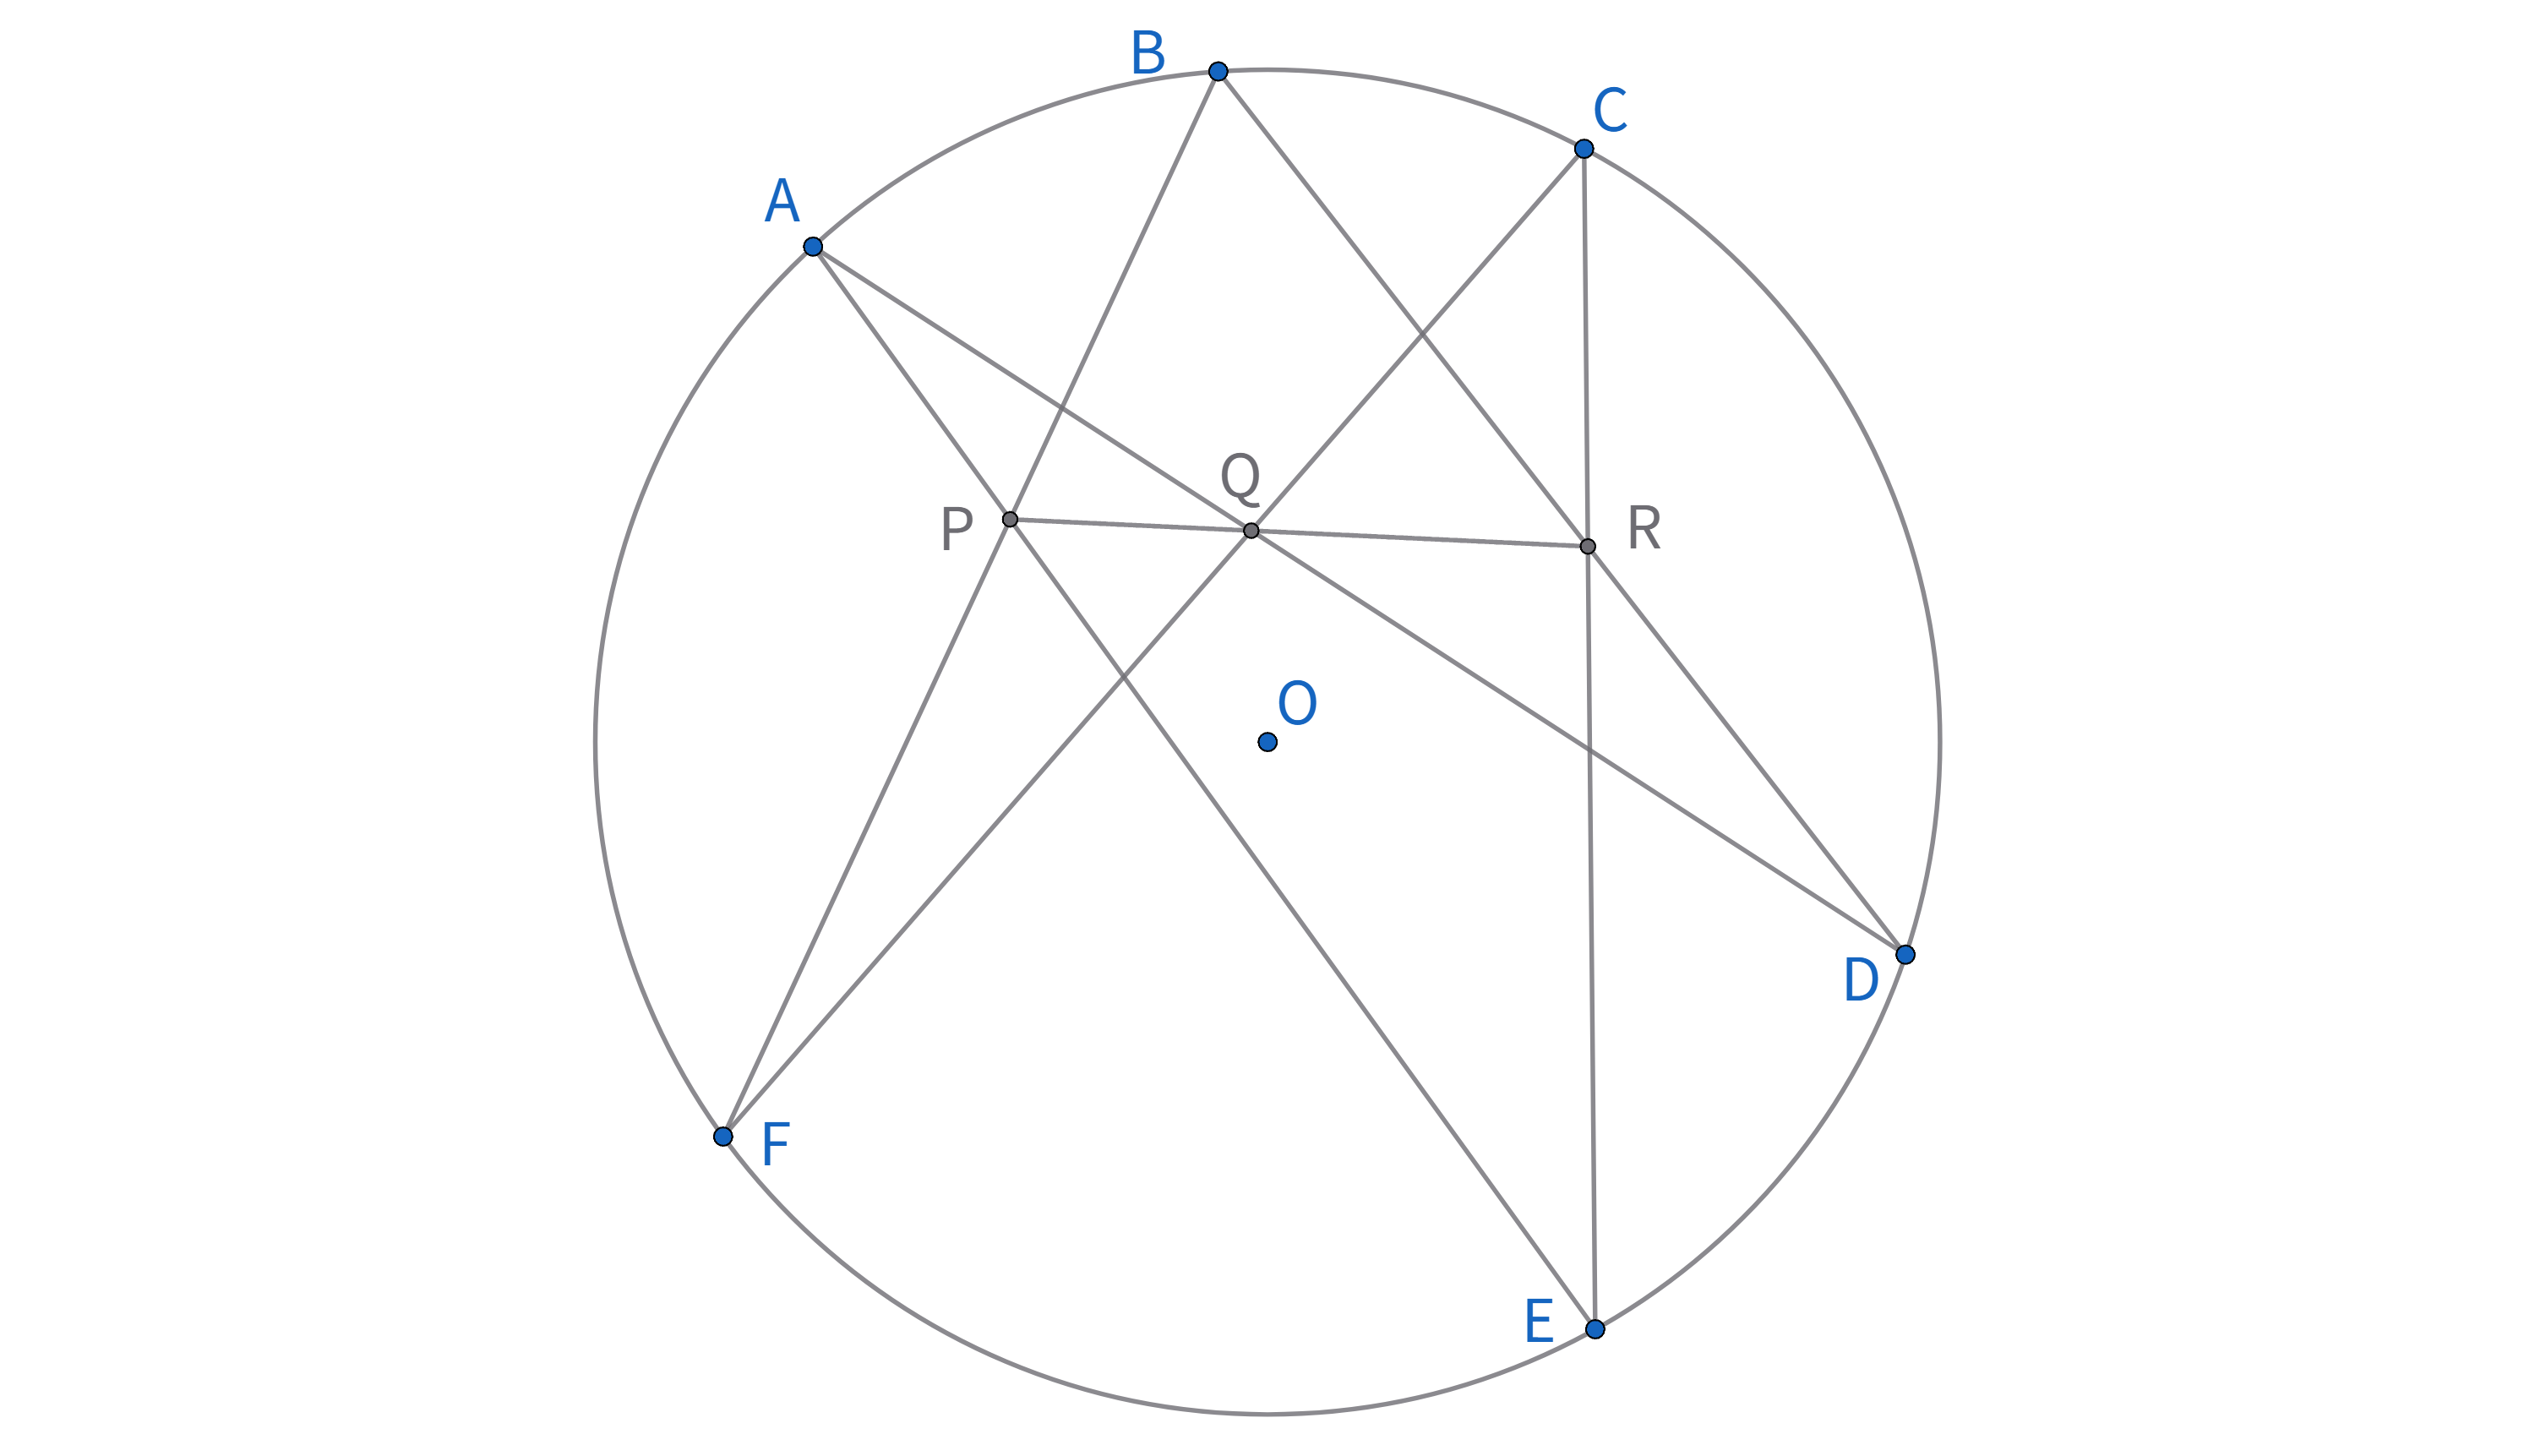
\includegraphics[width=\linewidth]{figures/帕斯卡定理.png}
    \caption{帕斯卡定理}
\end{figure}


%---------------------------------------------------
\newpage
\subsection{勒莫恩定理}
\begin{theorem}[勒莫恩(Lemoine)定理]
过$\triangle ABC$的三个顶点A、B、C作它外接圆O的切线,分别和BC、CA、AB所在直线交于D、E、F,则D、E、F三点共线。
\end{theorem}
\begin{figure}[htbp]
    \centering
    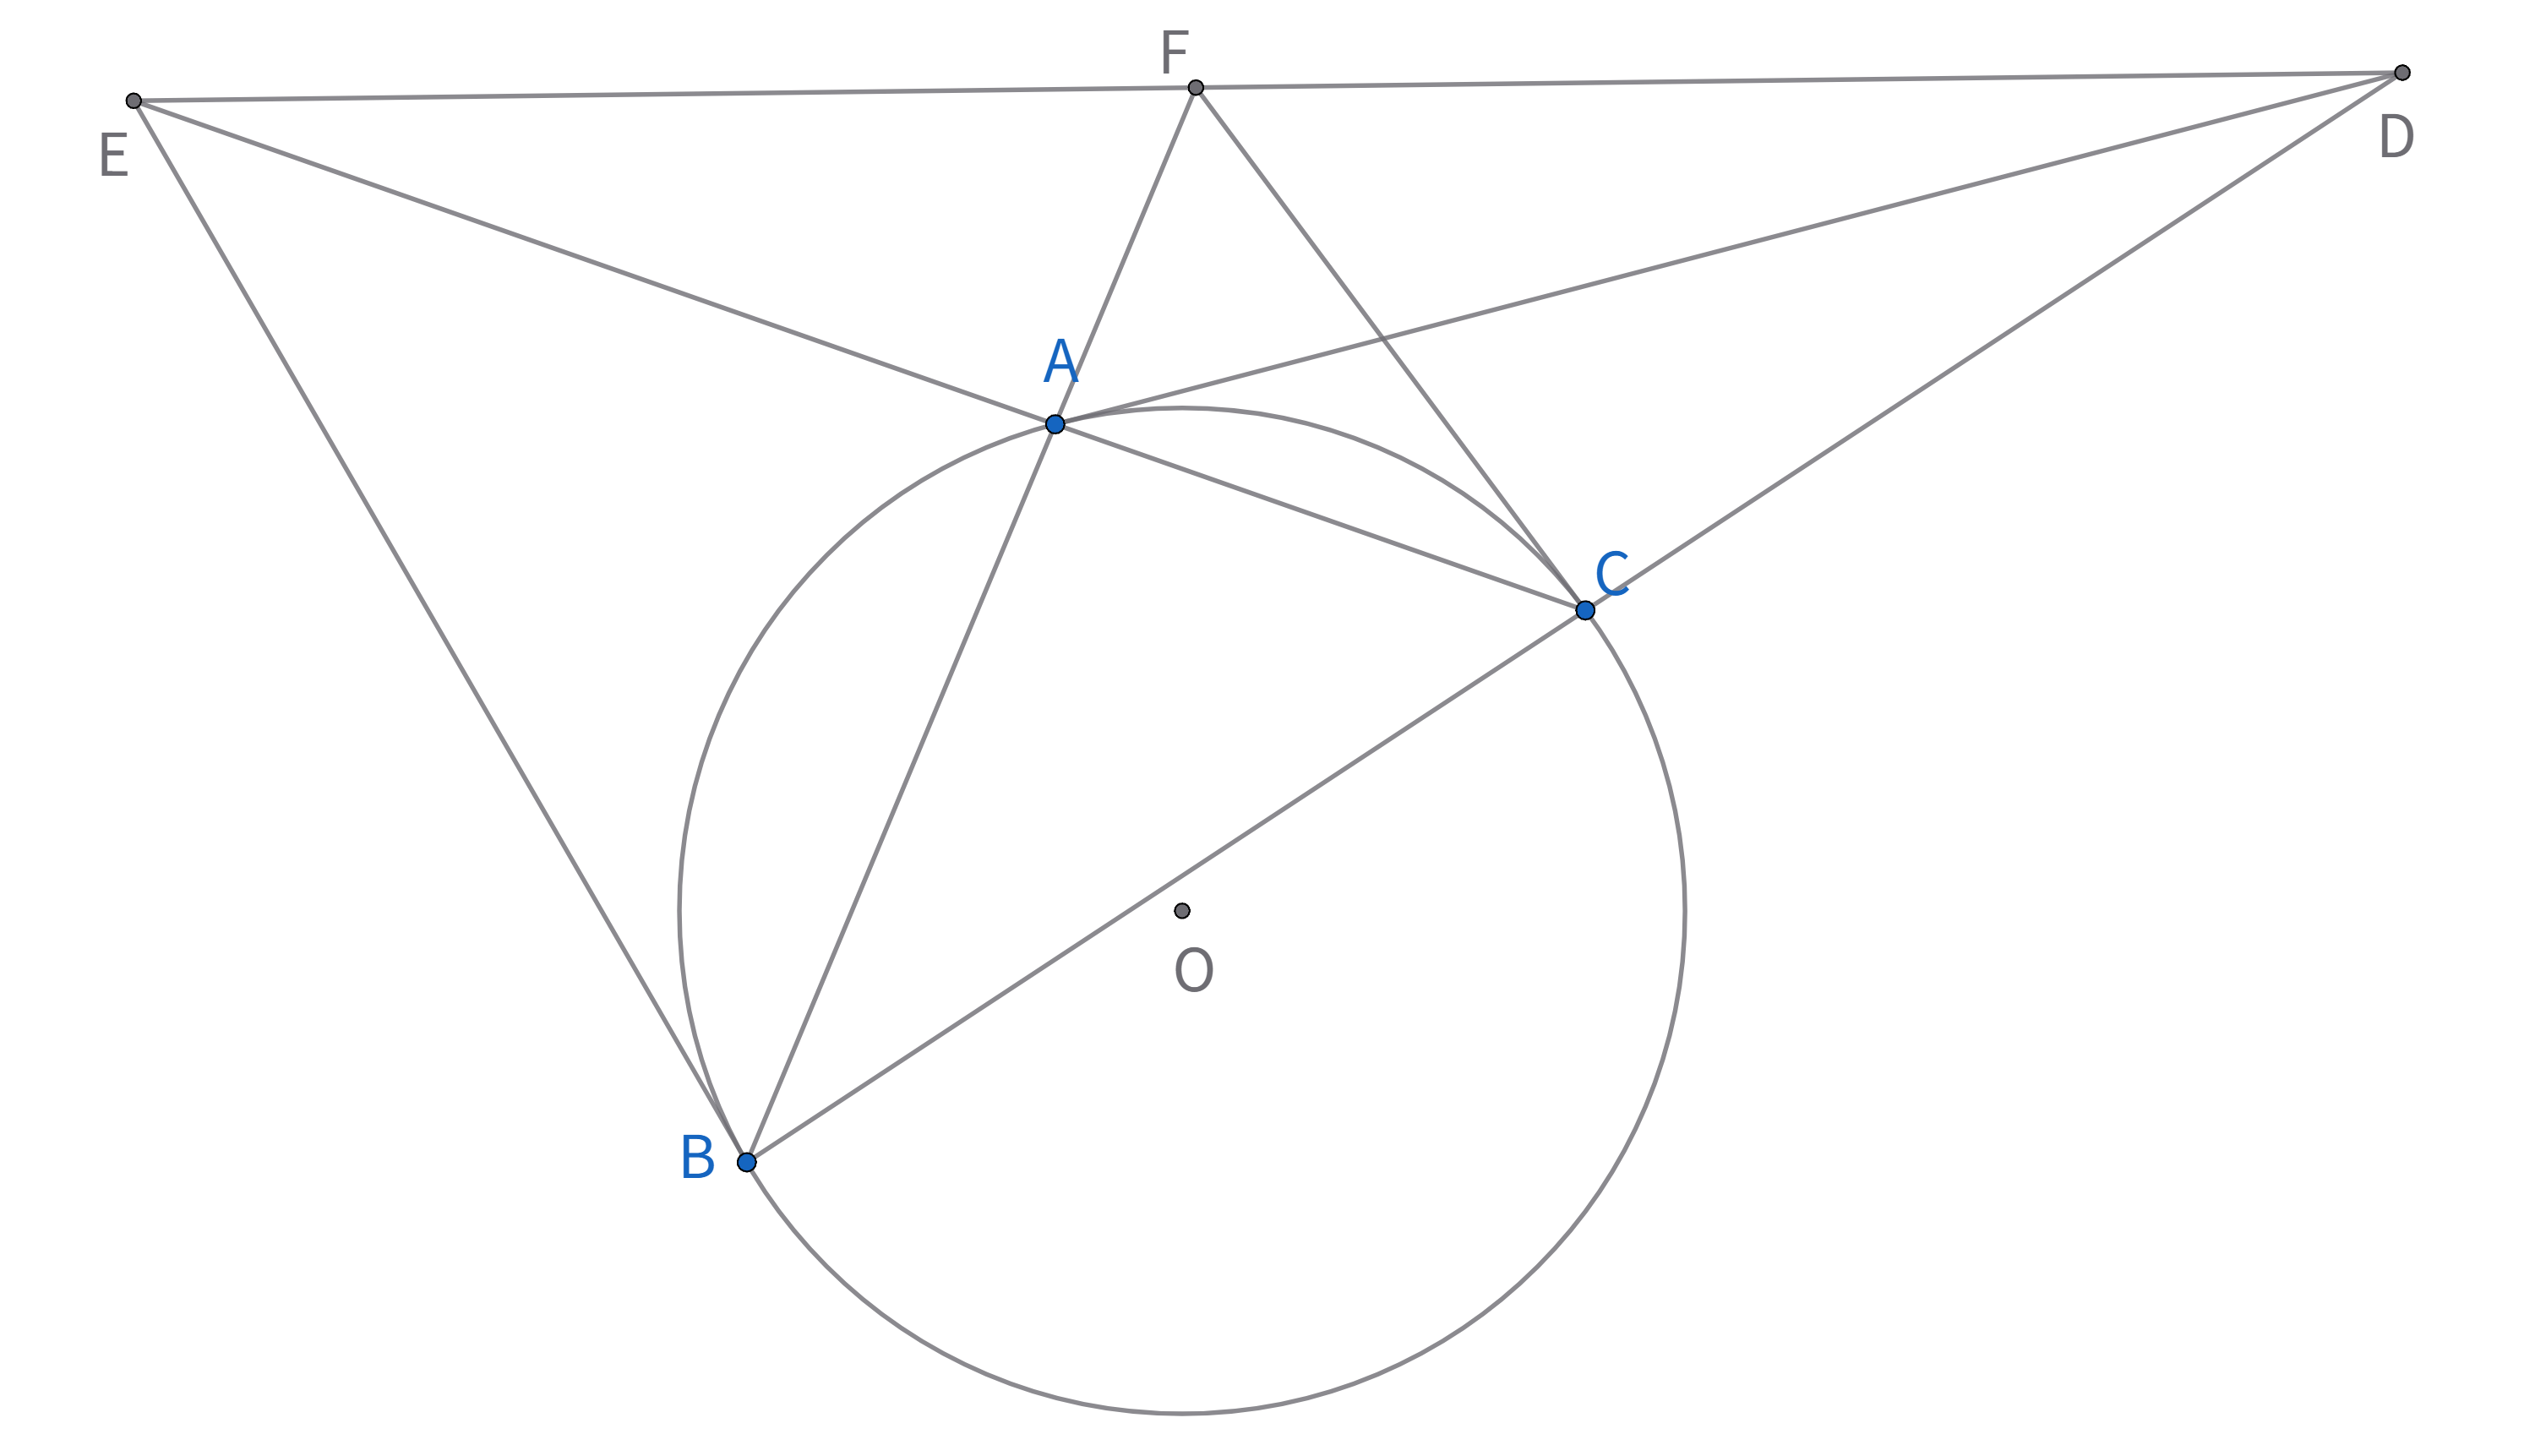
\includegraphics[width=\linewidth]{figures/勒莫恩定理.png}
    \caption{勒莫恩定理}
\end{figure}


%---------------------------------------------------
\newpage
\subsection{笛沙格定理}
\begin{theorem}[笛沙格(Desargues)定理]
若$\triangle ABC, \triangle DEF$ 的对应顶点连线共点(此点称为透视中心),则其对应边的交点一定共线(此线称为透视轴)。
此定理的逆定理亦成立。
满足德萨格定理的两个三角形称为透视的。
\end{theorem}
\begin{figure}[htbp]
    \centering
    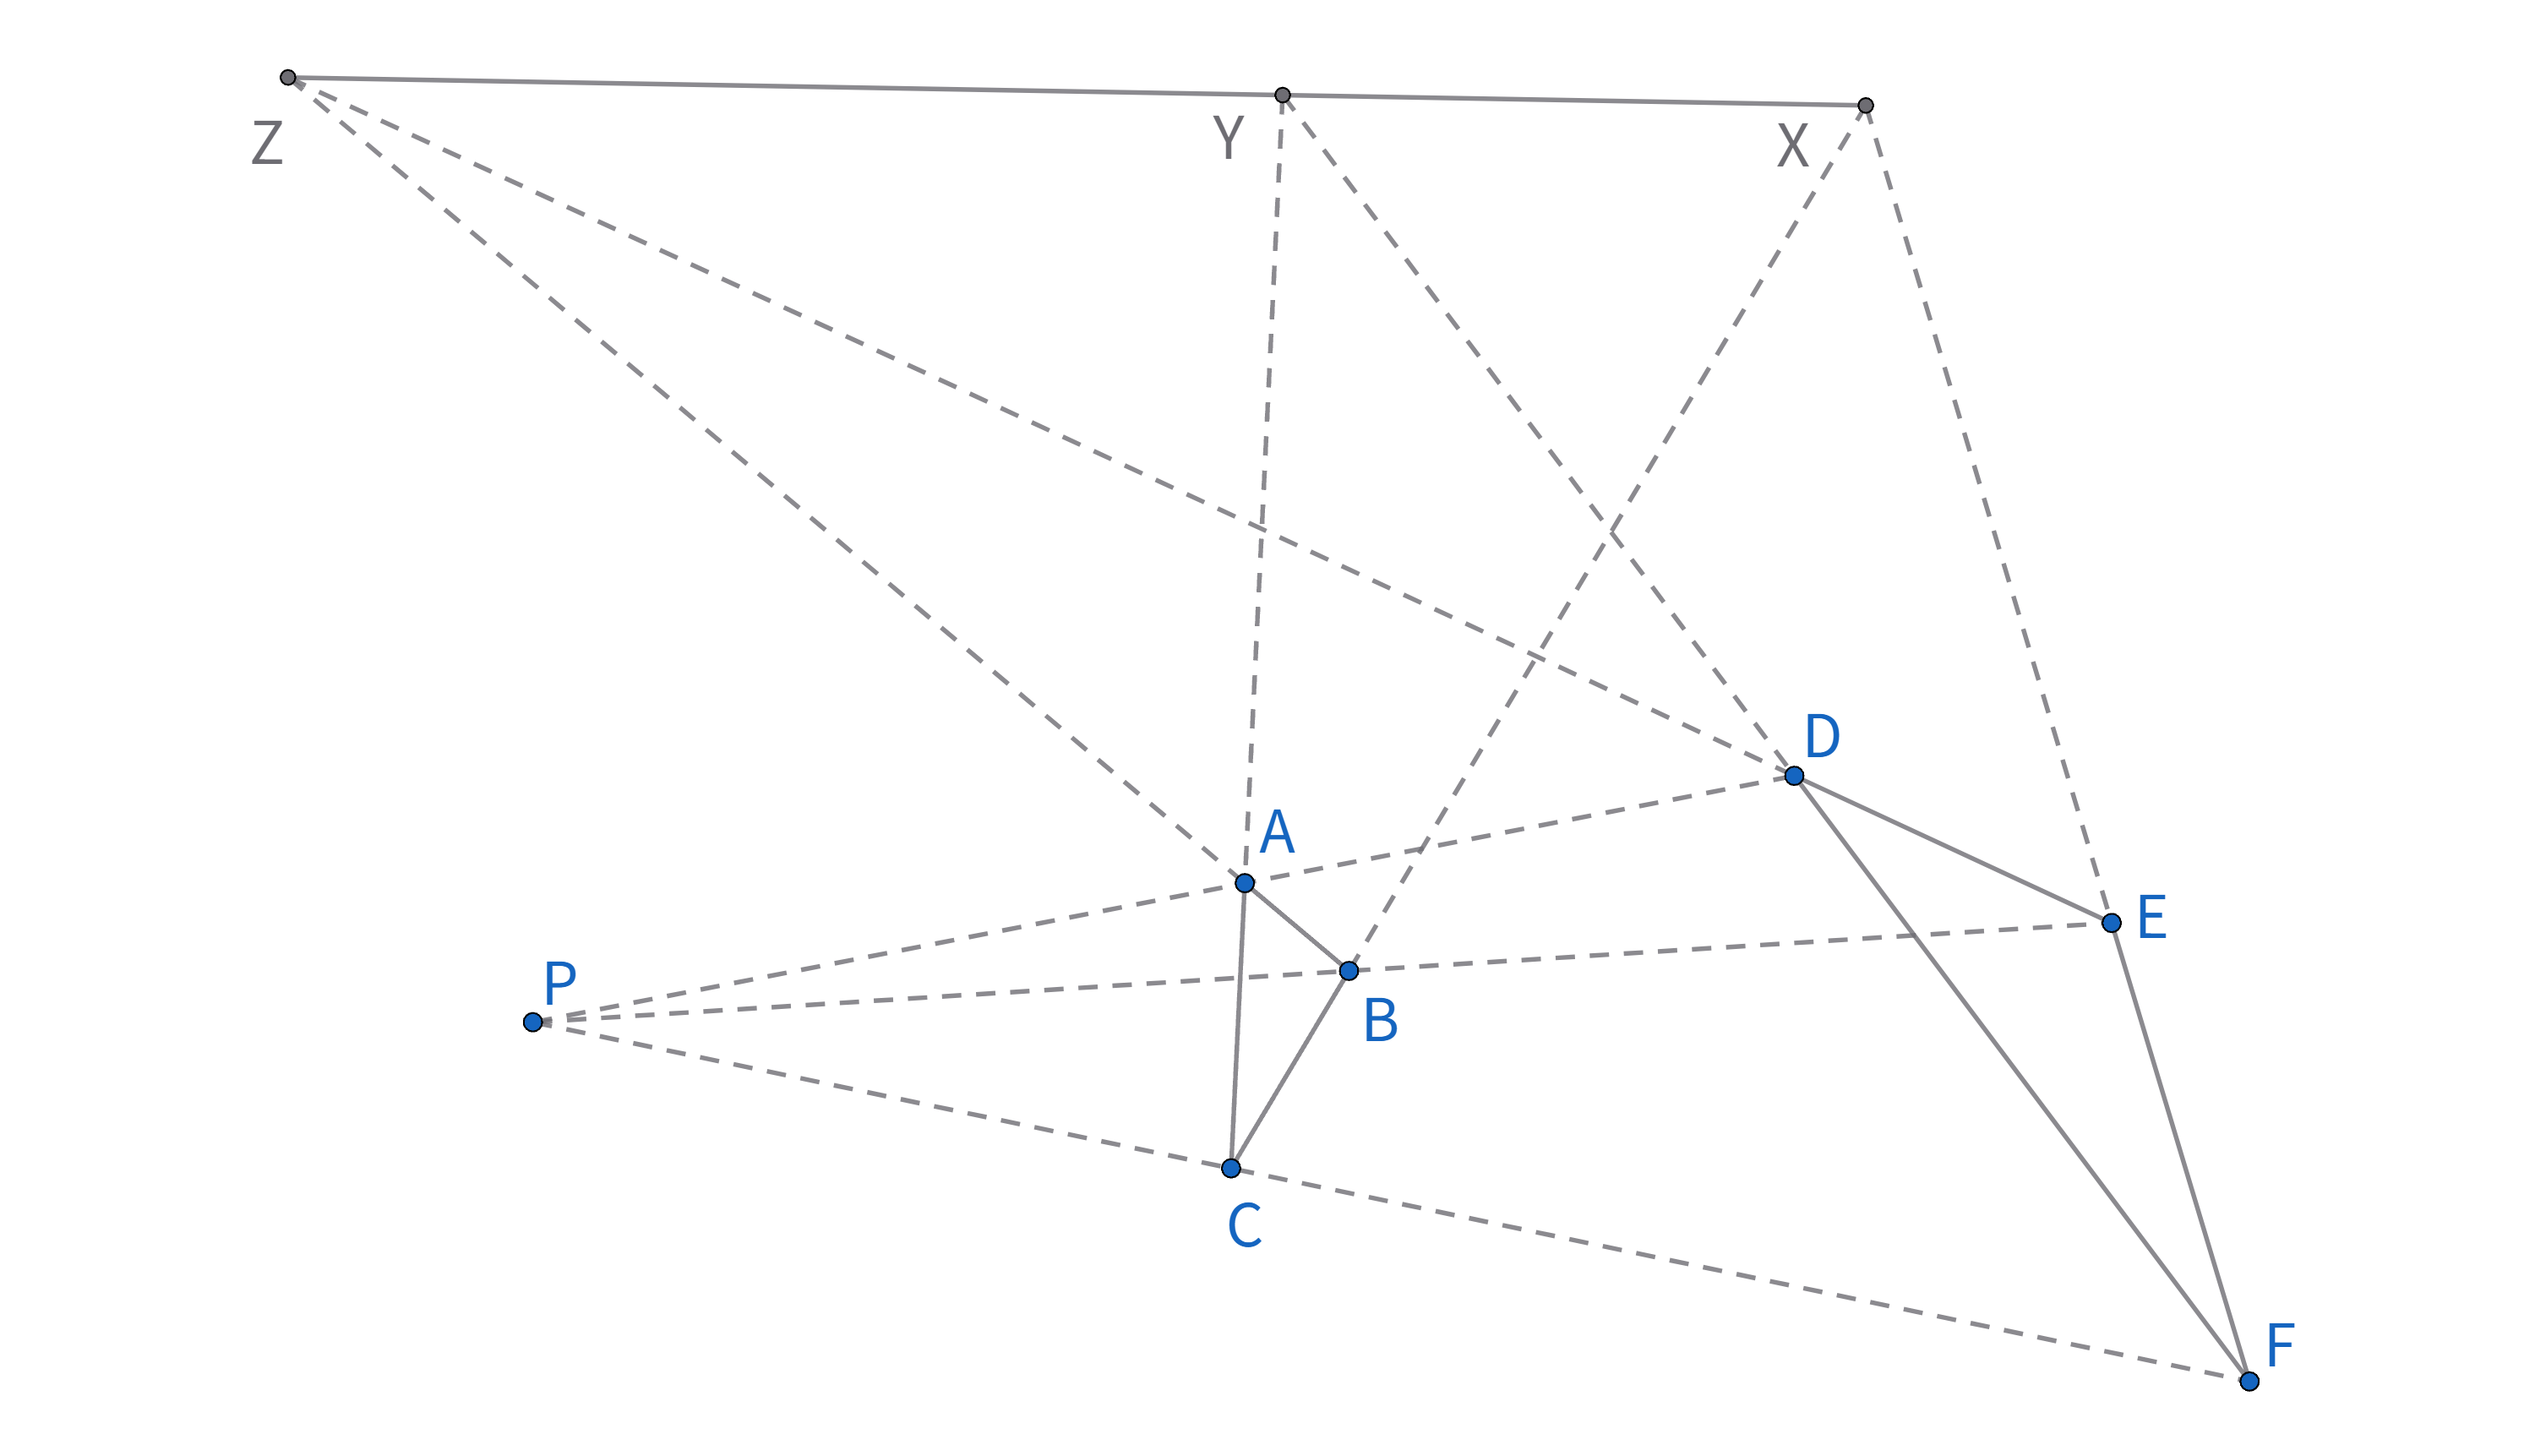
\includegraphics[width=\linewidth]{figures/笛沙格定理.png}
    \caption{笛沙格定理}
\end{figure}


%---------------------------------------------------
\newpage
\subsection{布拉美古塔(婆罗摩笈多)定理}
\begin{theorem}[婆罗摩笈多(Brahmagupta)定理]
圆内接四边形ABCD的对角线相互垂直,交点为M。过M做BC垂线交BC于点E,交AD于点F,则F是AD的中点。
\end{theorem}
\begin{figure}[htbp]
    \centering
    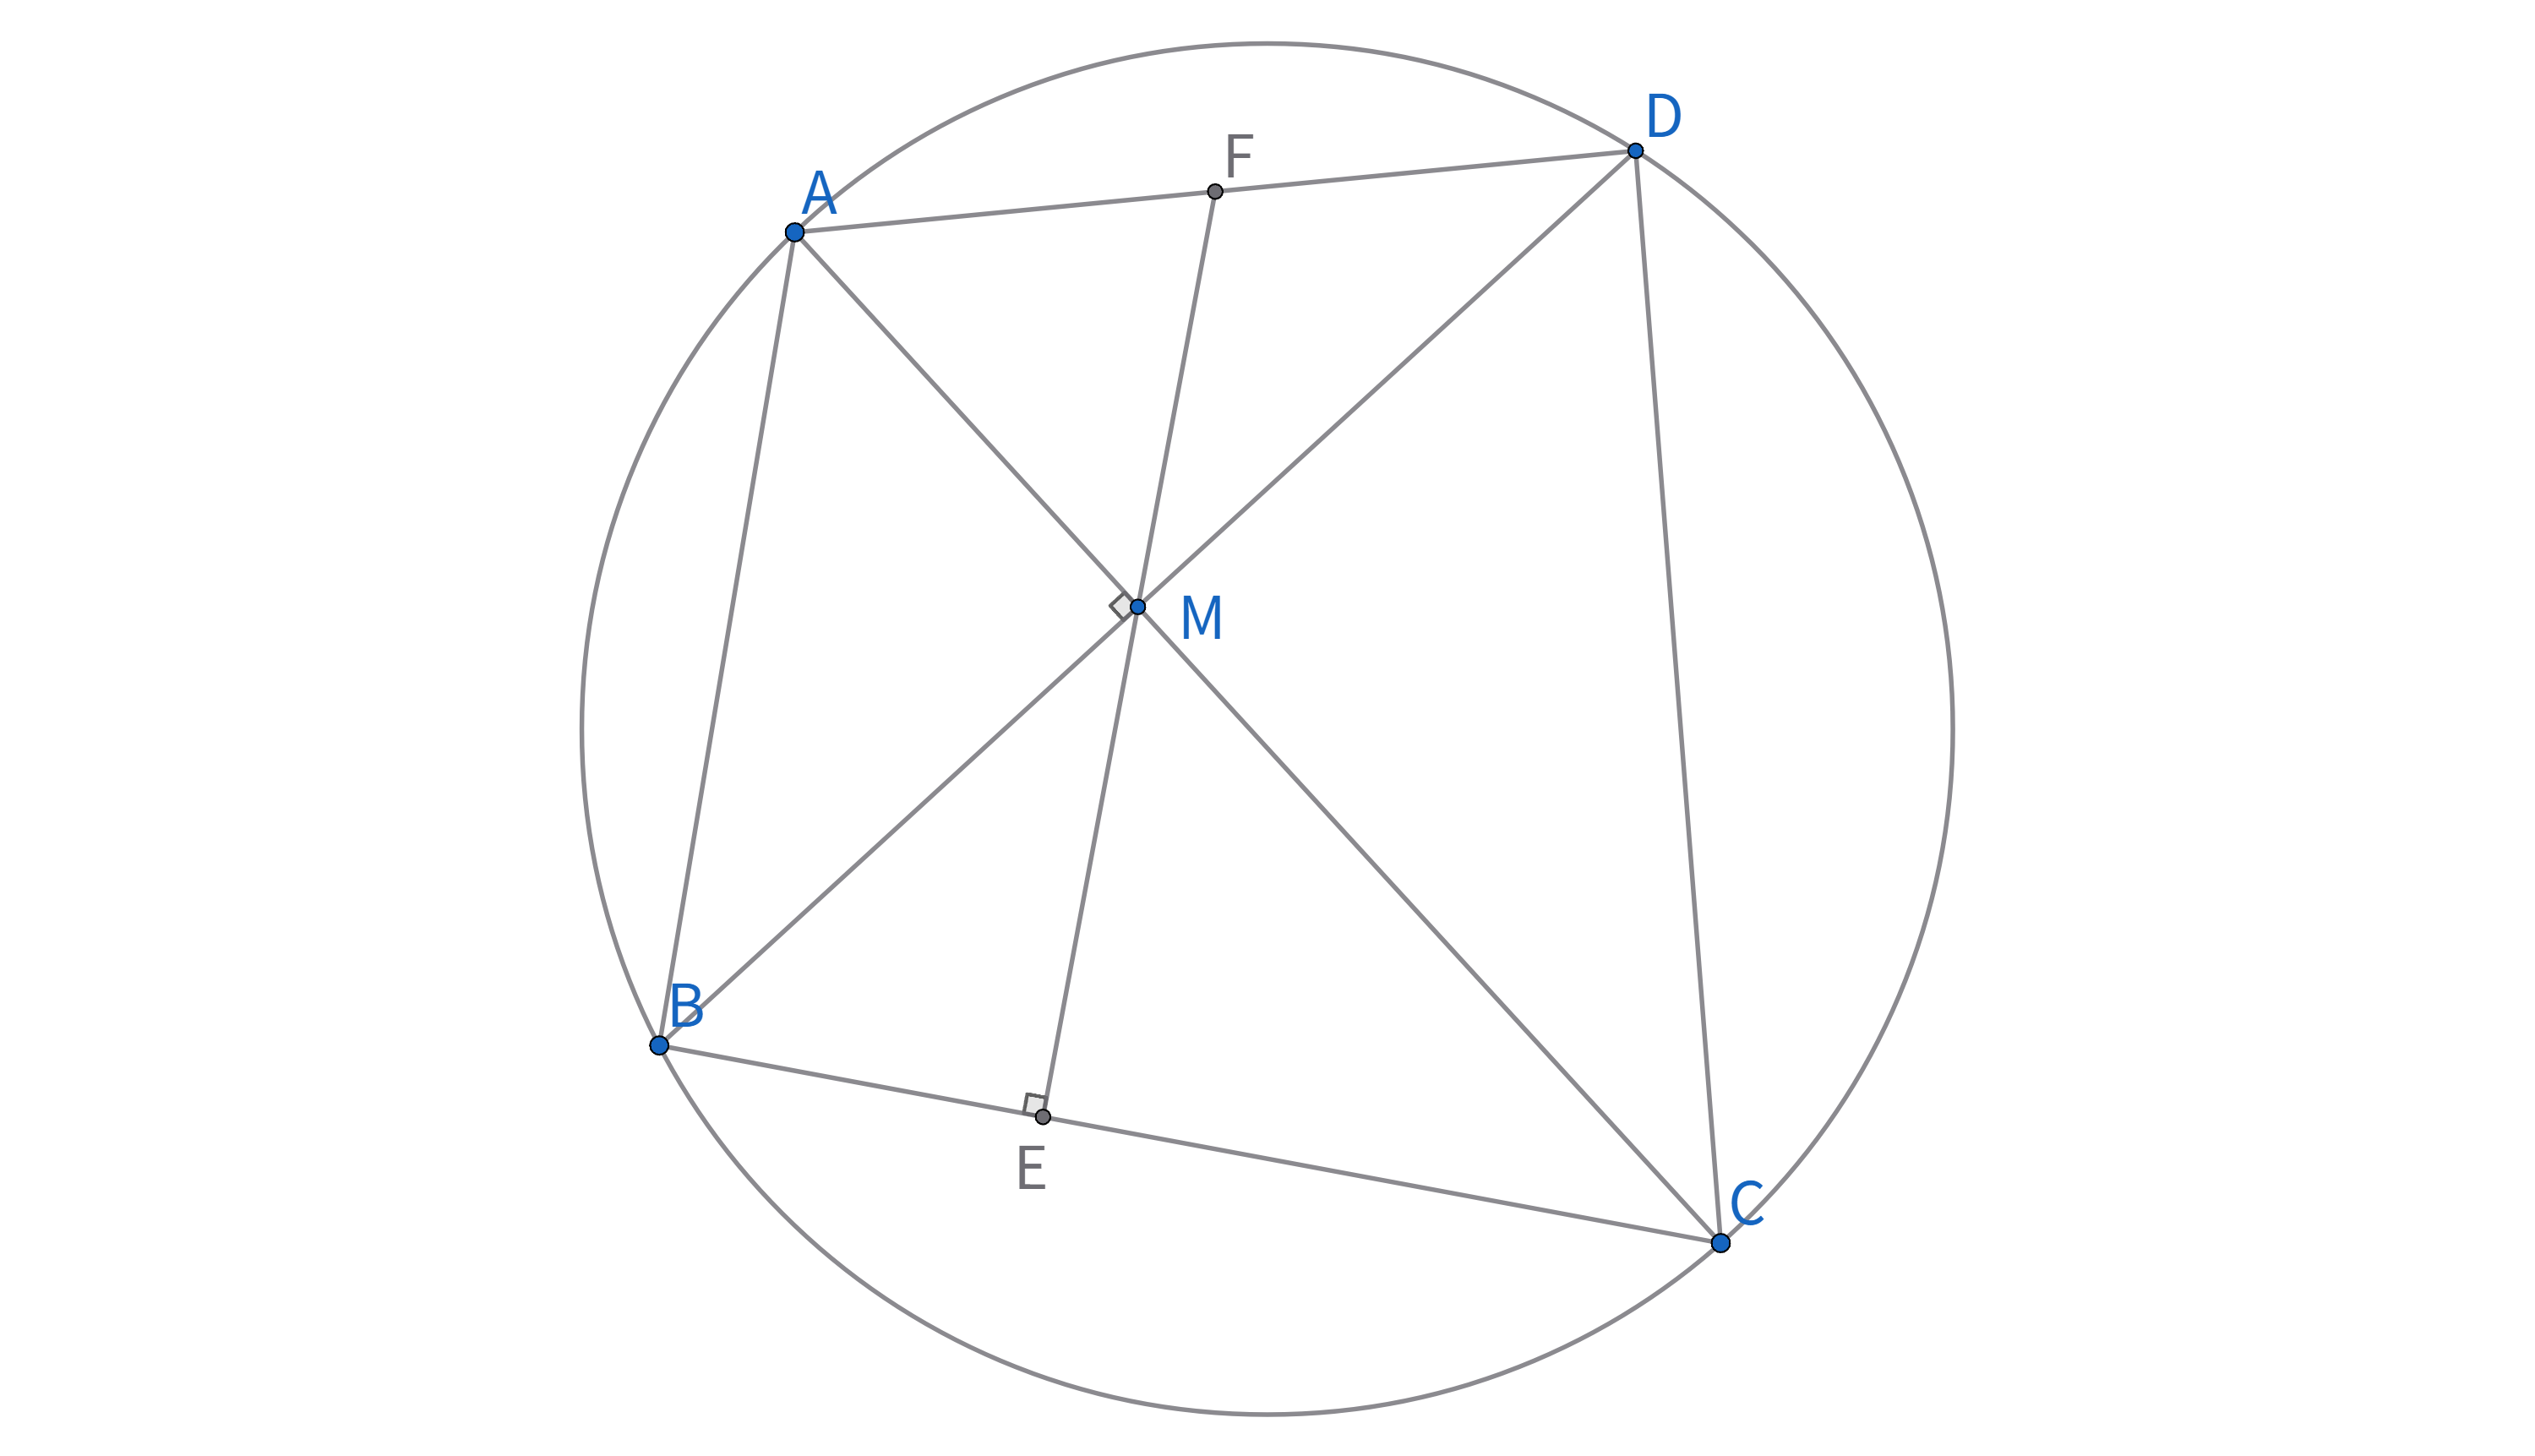
\includegraphics[width=\linewidth]{figures/婆罗摩笈多.png}
    \caption{婆罗摩笈多定理}
\end{figure}



%---------------------------------------------------
\newpage
\subsection{牛顿定理}
\begin{theorem}[牛顿(Newton)定理]
圆的外切四边形的对角线交点与对边切点连线交于一点。
\end{theorem}
\begin{figure}[htbp]
    \centering
    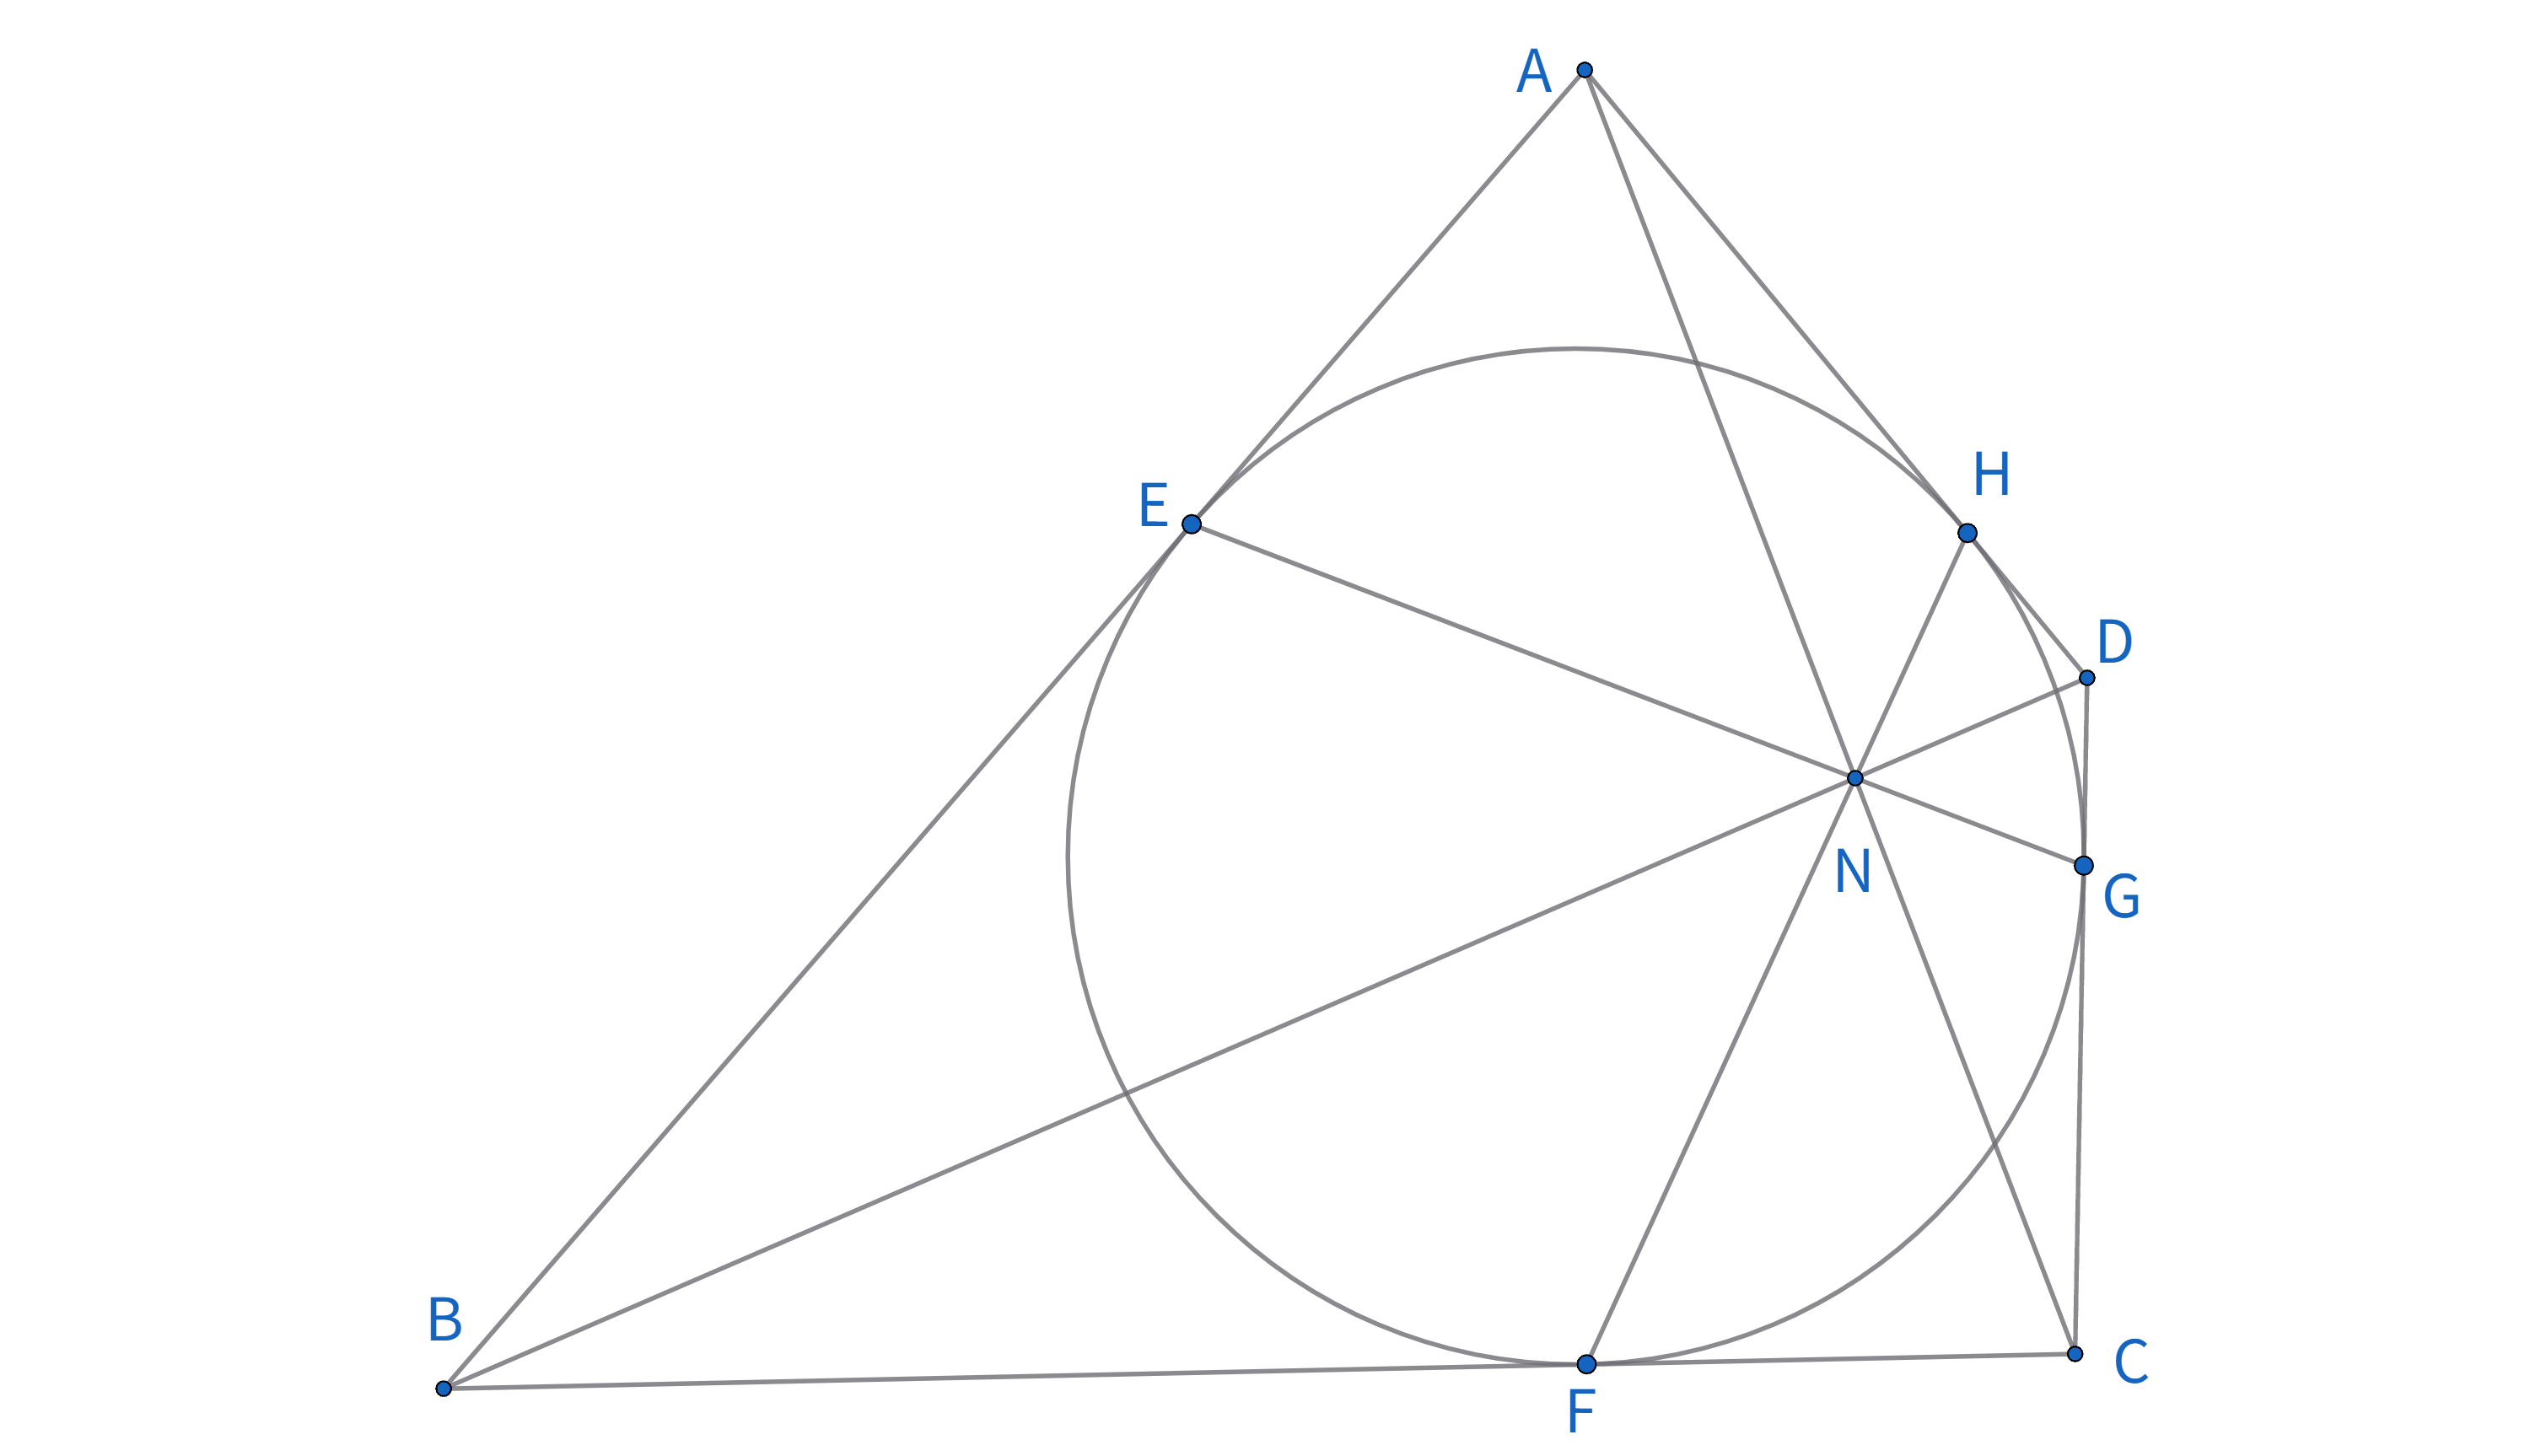
\includegraphics[width=\linewidth]{figures/牛顿定理.png}
    \caption{牛顿定理}
\end{figure}




%---------------------------------------------------
\newpage
\subsection{布利安香定理}
\begin{theorem}[布利安香(Brainchon)定理]
若一个六边形的六条边均与同一圆锥曲线相切,则该六边形的三条主对角线共点,该交点称为布列安桑点。\end{theorem}
\begin{figure}[htbp]
    \centering
    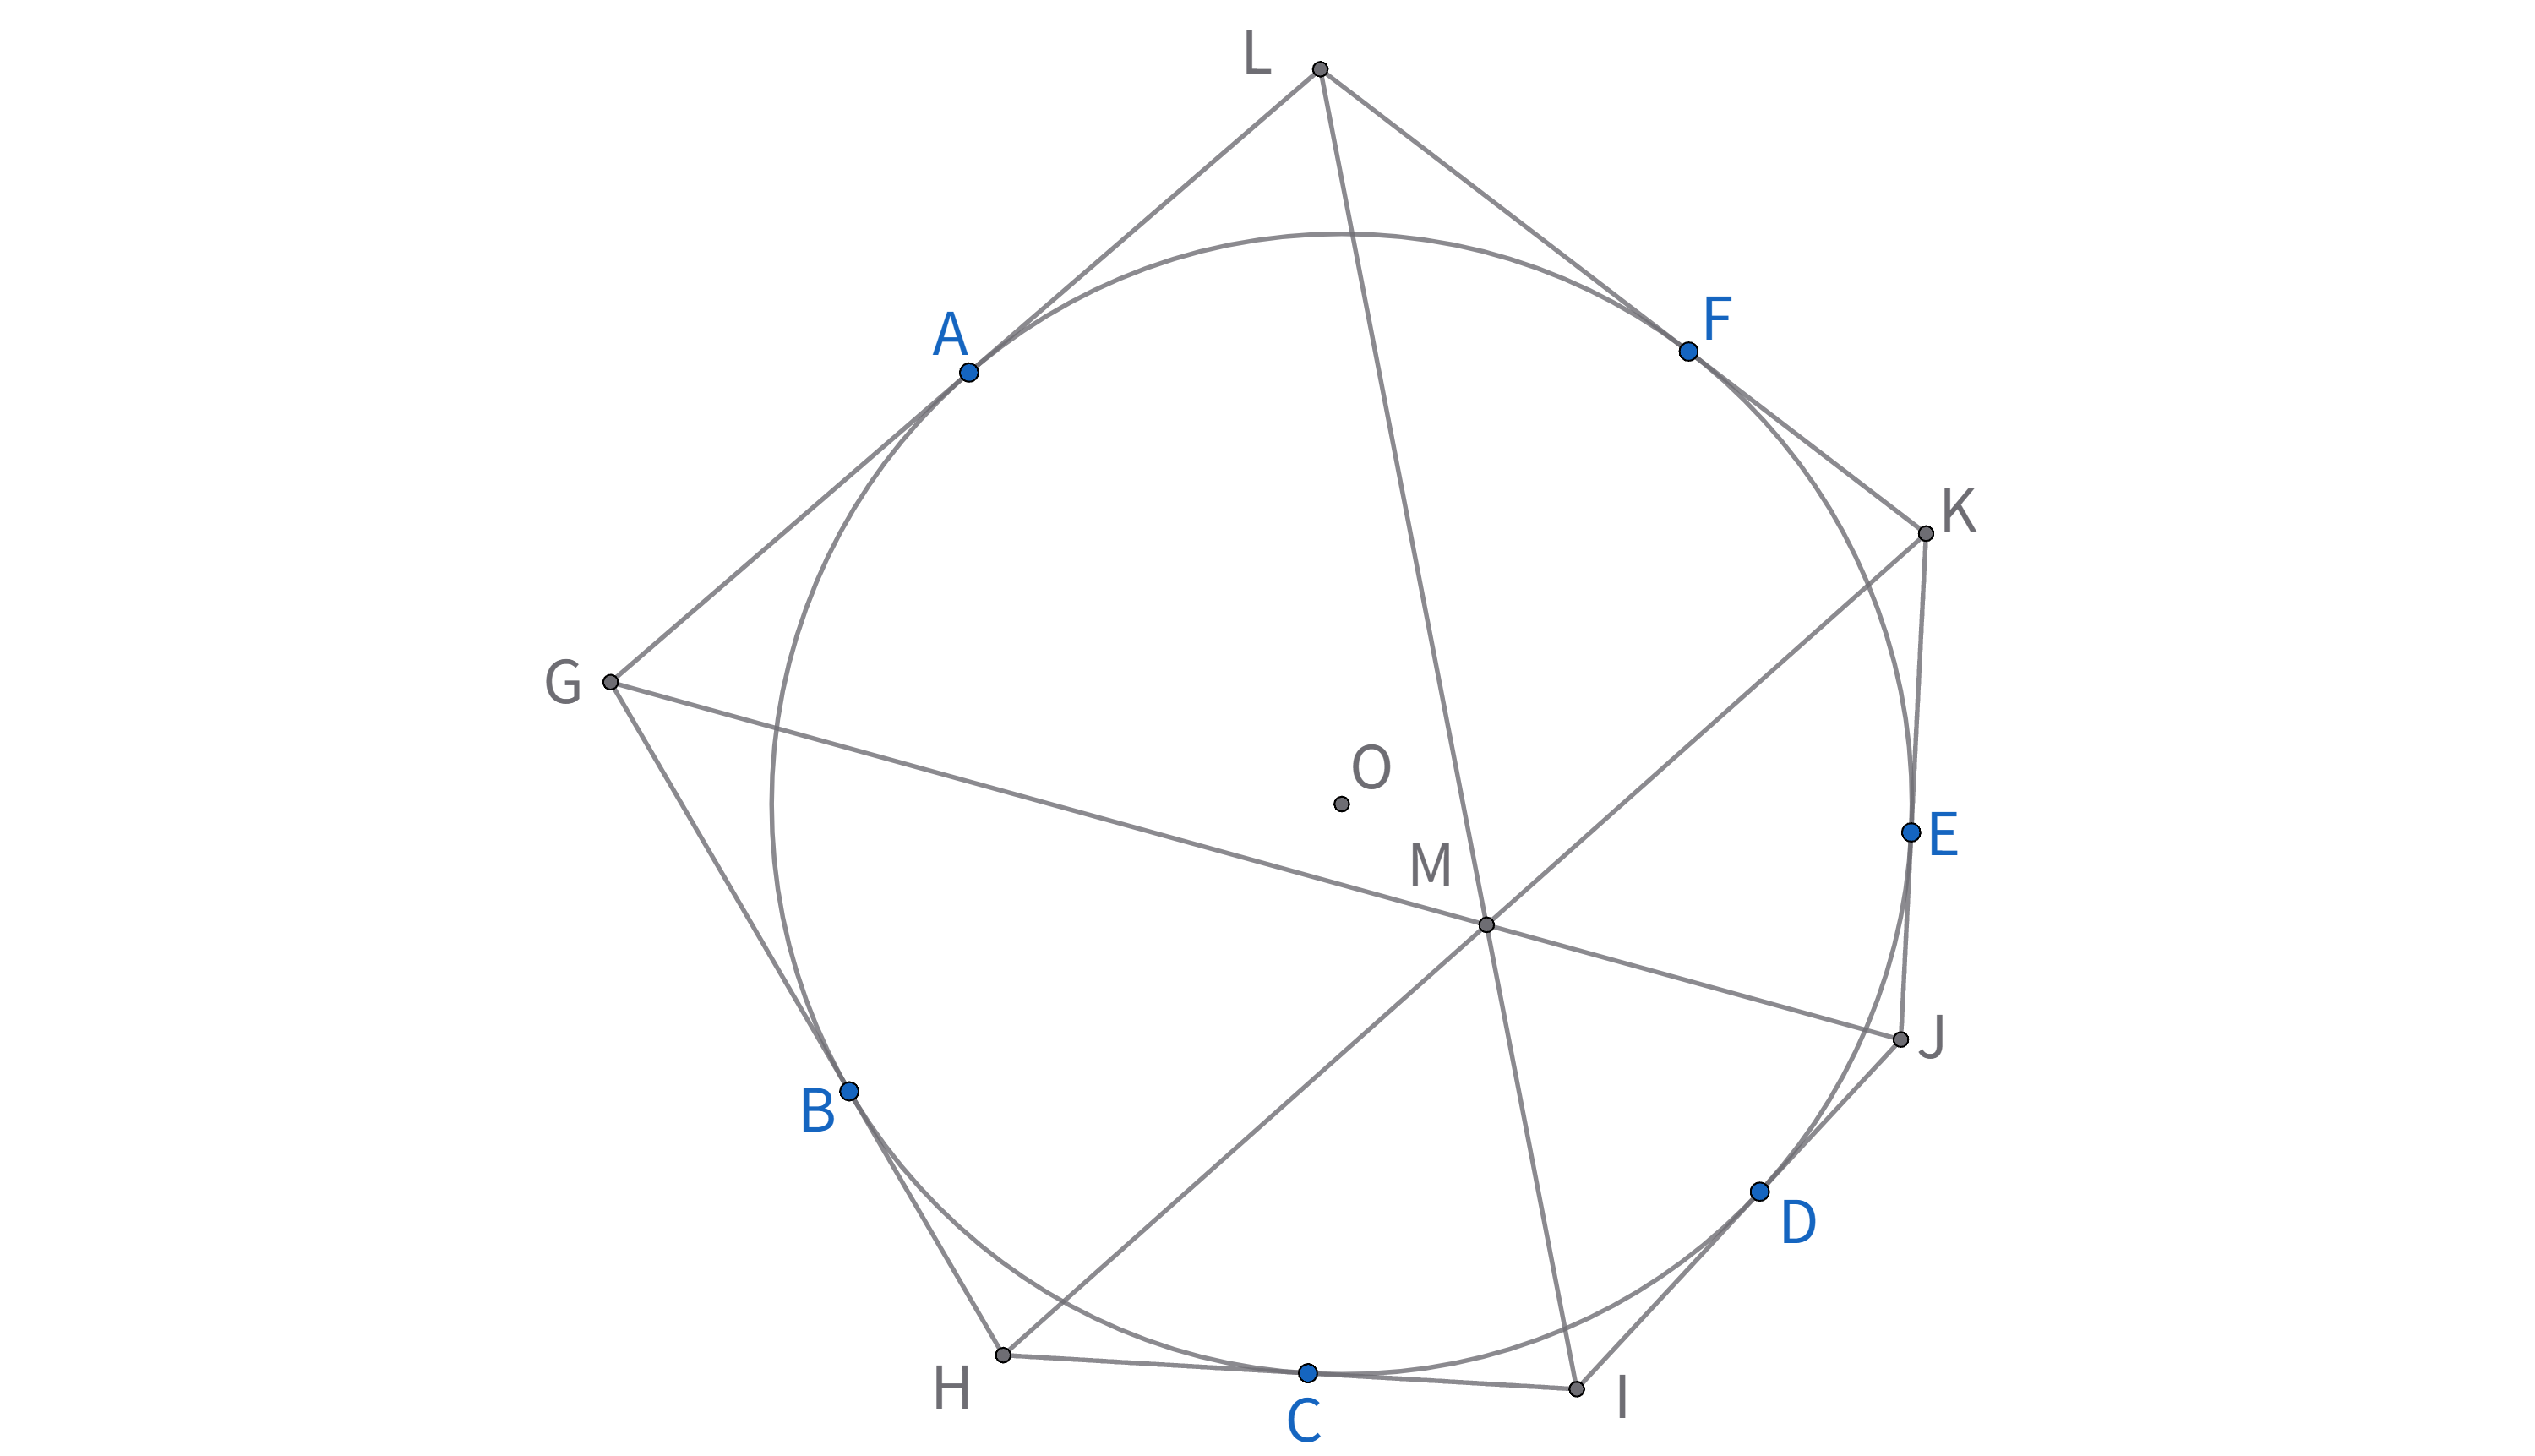
\includegraphics[width=\linewidth]{figures/布利安香.png}
    \caption{布利安香定理}
\end{figure}


